\documentclass[a4paper,14pt,russian]{article}
\usepackage[utf8]{inputenc}
\usepackage[T2A]{fontenc}      %% 2
\usepackage[russian]{babel}    %% 3
\usepackage{epstopdf}
\usepackage{graphicx}
\usepackage[Bakalavr]{ptvstyle}
%\renewcommand{\to}[0]{\xrightarrow[n \to \infty]{}}
\title{Оценивание эффективных доз в зависимости <<доза-эффект>>}
\author{студент группы 8403 \\ Кочеганов В.М.}
\advisor{д.ф.-м.н., профессор \\ Тихов М.С.}
\chief{д.ф.-м.н., профессор \\ Федоткин М.А.}
\date{2011}
\allowdisplaybreaks
\begin{document}
\maketitle
\numberwithin{equation}{subsection}
\tableofcontents

\newpage

\section*{Аннотация}
% Не удаляйте следующую строчку!
\addcontentsline{toc}{section}{Аннотация}
%
В работе предложены оценки категорий эффективных доз в зависимости <<доза-эффект>>. Доказана их состоятельность и асимптотическая нормальность. Для выборок конечного объема проведен компьютерный анализ рассматриваемых оценок.

Результаты работы опубликованы в журнале <<Обозрение прикладной и промышленной математики>> (см. \cite{Kocheganov1},\cite{Kocheganov2}).
\newpage
\section*{Введение}
% Не удаляйте следующую строчку!
\addcontentsline{toc}{section}{Введение}
% Не удаляйте следующую строчку!

Во многих областях медицины и биологии (фармакологии, токсикологии, радиобиологии, биохимии и др.) фундаментальной проблемой является изучение механизмов действия лекарственных средств, токсических веществ, ионизирующей радиации на биологические, экологические объекты. Наиболее востребовано решение данной проблемы в фармакологии при создании новых лекарственных средств (т.е. фармакологических средств, прошедших клинические испытания), поэтому при разработке новых лекарств анализ связи между дозой и эффектом и ее количественное определение имеет большое значение для практики. Несмотря на то, что спектр проявлений токсического процесса определяется строением токсиканта, тем не менее, выраженность развивающегося эффекта является функцией количества действующего агента. Для обозначения количества вещества, воздействующего на биологический объект, используется понятие доза. Под дозой понимается некоторое количественное значение агента (фактора), изменяющее состояние исследуемого объекта на введенную дозу.

В некоторых случаях (например, при статистической оценке возраста менархе или возраста менопаузы, см.~\cite{Fin}, когда фиксируется возраст пациента и наличие или нет интересующего нас события, точный момент наступления которого неизвестен) отсутствует понятие дозы в вышеопределенном смысле, тем не менее, задача оценки возраста менархе или оценки возраста менопаузы укладывается в рассматриваемую в работе модель доза-эффект.

На современном этапе в токсикометрии востребованными являются величины доз, которые вызывают появление эффекта, учитываемого в экспериментальной группе тест-объектов с заданной вероятностью $0.01$; $0.05$; $0.1$; $0.16$;
$0.5$; $0.84$; $0.9$; $0.95$; $0.99$. Такие дозы получили название доз $ED_1$, $ED_5$, $ED_{10}$, $ED_{16}$,  $ED_{50}$, $ED_{84}$, $ED_{90}$,  $ED_{95}$, $ED_{99}$. Поэтому как среднеэффективная доза $ED_{50}$, так и другие категории доз: малые  $(ED_1, ED_5, ED_{10}, ED_{16})$ и большие $(ED_{84}, ED_{90},  ED_{95}, ED_{99})$ дозы , должны в полной мере отвечать максимально жестким критериям корректности, надежности, адекватности и состоятельности.

В предложенной работе нас интересует проблема нахождения граничных (малых и больших) эффективных доз, для решения которой использованы оценки квантилей распределения, основанные на непараметрической оценке Надарая-Ватсона.

\newpage

\section{Постановка задачи}

Рассмотрим следующую математическую модель зависимости <<доза-\linebreak эффект>>.

Пусть в биообъект вводится доза $U$ и наблюдается альтернативный ответ $W$. Основу модели составляет предположение, что существует латентная величина $X$ --- пороговая доза, --- являющаяся самой большой дозой, при которой не наблюдается эффекта в эксперименте. Для каждого биообъекта эта доза будет различной, что определяется индивидуальной чувствительностью особей биологического вида к тестируемому препарату. Однако в однородно массе величина $X$ будет случайной величиной.

Пусть $\{ ( X_i, U_i ), 1\leq i\leq n \}$ --- потенциальная повторная выборка, вместо которой наблюдается выборка ${\mathcal U}^{(n)}=\{ (U_i, W_i)$, $1\leq i\leq n \}$, где $W_i=I(X_i<U_i)$ есть индикатор события $\left\{X_i<U_i\right\}$. Здесь  $U_i$ рассматриваются как вводимые дозы, а $W_i$ --- как  эффект от воздейcтвия этой дозы ($U_i$) на биообъект.

Как правило, модель зависимости <<доза-эффект>> предполагает величины $U_i$ случайными (случайный план эксперимента), однако в некоторых случаях вводимые дозы известны заранее и, следовательно, могут рассматриваться как детерминированные величины. В данной работе рассматривается последний случай, называемый также фиксированным планом эксперимента.


Случайные величины $X_i$ имеют функцию распределения $F(x)$, которую будем предполагать абсолютно непрерывной: $F(x)=\int _{-\infty }^{x}f(t)\,dt$, причем $f(t)>0$.

%Требуется оценить функцию распределения $F(x)$ и по ней построить оценку $\hat{x}_\la$ квантиля %порядка $\la$ (этого же распределения $F(x)$) $x_\la = \Fb(\la) = ED_{100\la}$, $0<\la<1$.

\newpage

\section{Исходные предположения}
\numberwithin{equation}{section}
В данном пункте определены оценки квантилей распределения, анализ асимптотического поведения которых составляет содержание данной работы. Здесь  также опишем условия на введенные в модели математические объекты, в которых будем проводить дальнейшие выкладки.

Пусть $\brrr{X_i,\ i=1,\ldots,n}$ --- последовательность независимых одинаково распределенных на отрезке $[0,1]$ случайных величин с функцией распределения $F(x)$, а $P = \{u_1,\ \ldots,\ u_n\}$ --- совокупность точек разбиения отрезка $[0,1]$, $0 < u_1 < \ldots < u_n < 1$.

Для оценки функции $F(x)$ будем использовать статистику, аналогичную статистике Надарая-Ватсона,
\begin{equation}\label{Fn}
F_{n h_r}(x) = \frac{1}{n h_r} \sum_{i=1}^{n} K_r \br{\frac{x-u_i}{h_r}}W_i,
\end{equation}
где $W_i=I(X_i<u_i)$ и $K_r(x)$ --- финитная ядерная функция, т.е. является симметричной плотностью с компактным носителем.

Для оценок квантиля порядка $\la$ распределения $F(x)$ будем использовать следующие статистики:
\begin{align}
\hat{x}_{1,\la} &= \frac{1}{n h_d} \sum_{i=1}^n \int_{-\infty}^\la
K_d\br{\frac{F_{n h_r}\br{i/n}-u}{h_d}}du;
\label{xla1}\\
\hat{x}_{2,\la} &= \frac{ \sum_{i=1}^{n} K_d\br{\frac{F_{n h_r}(i/n)-\la}{h_d}}\frac{i}{n}}{ \sum_{i=1}^{n} K_d\br{\frac{F_{n h_r}(i/n)-\la}{h_d}}};
\label{xla2}\\
\hat{x}_{3,\la} &= \frac{ \sum_{i=1}^{n} \I{-\infty}{\la} K_d\br{\frac{F_{n h_r}(i/n)-u}{h_d}}\frac{i}{n}du}{\sum_{i=1}^{n} \I{-\infty}{\la} K_d\br{\frac{F_{n h_r}(i/n)-u}{h_d}}du};
\label{xla3}\\
\hat{x}_{4,\la} &= F_{nh_r}^{-1}(\la).
\label{xla4}
\end{align}

Функция $K_d(x)$ является финитным ядром; величины $h_r=h_r(n)$ и $h_d=h_d(n)$ --- сглаживающие параметры, они неслучайны и зависят от объема выборки $n$. Параметры $h_r$ и $h_d$ носят также название ширины окна просмотра данных.

\begin{remark}
  Оценка \eqref{xla1} была заимствована у H.~Dette из \cite{Dette} с некоторыми изменениями. Именно, в качестве оценки функции распределения в работе H.~Dette была использована локальная оценка функции регрессии.

  Основная идея самой оценки состоит в следующем.
  Суммирование в оценке \eqref{xla1} является приближением интеграла
  $$
  \frac{1}{ h_d} \I{0}{1}\int_{-\infty}^\la
K_d\br{\frac{F_{n h_r}\br{x}-u}{h_d}}dudx.
  $$
  Далее, если заменить $F_{n h_r}\br{x}$ на оцениваемую функцию распределения, то получим следующее выражение:
  $$
   \frac{1}{ h_d} \I{0}{1}\int_{-\infty}^\la
K_d\br{\frac{F\br{x}-u}{h_d}}dudx = \I{0}{1} I\brrr{F(x)\leq \la}dx + o(1) = x_\la + o(1).
  $$
\end{remark}

Сформулируем исходные предположения.

\begin{itemize}
\item
Условия $(H)$ на сглаживающие параметры $h_r$ и $h_d$:
\begin{description}
{

\item[$\mathbf H_1:\;$]
$h_r \xrightarrow[n \to \infty]{} 0,\qquad h_d \xrightarrow[n \to \infty]{} 0;$

\item[$\mathbf H_2:\;$]
$ h_r/h_d \xrightarrow[n \to \infty]{} \infty;$
\item[$\mathbf H_3:\;$]
$n h_r^5 = O(1);$
\item[$\mathbf H_4:\;$]
$ 1\left/\br{n h_r h_d^{8/3}}\right.=o(1).$
}
\end{description}
Условия $(H)$ являются непротиворечивыми, поскольку последовательности $h_r = n^{-1/5}$ и $h_d=n^{-1/4}$ им удовлетворяют.
\item
Условия $(K)$ на ядерные функции $K_r(x)$ и $K_d(x)$:
\begin{description}

\item[$\mathbf K_1:$]
$\int_{-1}^1 K_{r,d}(x)dx=1.$

\item[$\mathbf K_2:$]
$K_{r,d}(x)\geq 0$, причем $K_{r,d}(x)=0,\ x \notin [-1,1]$;

\item[$\mathbf K_3:$]
$K_{r,d}(x)=K_{r,d}(-x),\ x \in \mathbb R;$

\item[$\mathbf K_4:$]
$K_r(x)$ и $K_d(x)$ являются непрерывно дифференцируемой и  четырежды непрерывно дифференцируемой на отрезке $[-1,1]$ функциями.
\item[$\mathbf K_5:$]
Являются конечными следующие величины:
\begin{align*}
\nu_r^2 &= \int K_r(z)z^2dz, & \hat{\nu}_r^2 &= \int K_r(z)z^4dz,\\ \nu_d^2 &= \int K_d(z)z^2dz, &\hat{\nu}_d^2 &= \int K_d(z)z^4dz
\end{align*}\label{nu}

\end{description}


\item
Условия $(F)$ на функцию распределения $F(x)$:
\begin{description}

\item[$\mathbf F_1:$]
$F(x)$ имеет четвертую непрерывную производную на [0,1];

\item[$\mathbf F_2:$]
$F'(x) = f(x)>0, \forall x \in [0,1]$, т.е. $F(x)$ возрастает на $[0,1]$.

\end{description}

\item
Условия $(P)$ на совокупность точек разбиения $P = \{u_1,\ldots,u_n\}$ отрезка $[0,1]$, $0 < u_1 < \ldots < u_n < 1$:
\begin{description}

\item[$\mathbf P:$]
Обозначим $u_0 = 0,~ u_{n+1}=1$, тогда предположим, что
$$\max_{k=\overline{0;n}}\max\brrr{\brrrr{u_k-\frac{k}{n}},\brrrr{u_{k+1}-\frac{k}{n}}}= O\br{\frac1n}.$$

Последнее условие фактически означает, что $u_k = \frac{k}{n} + O\br{\frac1n}$, где последовательность $n O\br{\frac1n}$ ограничена равномерно для всех $k = \overline{1,n}$.
\end{description}

\end{itemize}


Все приводимые утверждения в работе исходят из описанных в этом пункте условий (если не сделано иных оговорок), поэтому исходные предположения утверждений будем, как правило, опускать.
\newpage

\section{Вспомогательные утверждения}
\numberwithin{equation}{section}
В этом пункте представлены общие результаты, необходимые для изучения асимптотики введенных выше оценок \eqref{xla1} --- \eqref{xla4}.


Сначала предложим без доказательства утверждение из книги \cite{Monte}, позволяющее оценить интеграл от функции по ее значениям в конечном числе точек.
\begin{lemma}[Неравенство Koksma-Hlawka]\label{KH}
Если функция $g$ имеет ограниченное изменение в кубе $[0;1]^s$ и $P=\{u_1;\; \dots;\;u_n\}$ --- множество точек из $[0;1]^s$, то
$$\left|\frac1n \sum^n_{k=1}g(u_k) - \int\limits_{[0,1]^s}g(u)du\right| \leq D^*[P] V[g],$$
где
$$D^*[P]= \sup_{y_1, \ldots, y_s \in [0,1]}\brrrr{\frac{A(y_1, \ldots, y_s)}{n} - y_1 \cdot \ldots \cdot y_s},$$
$V[g]$ --- вариация функции $g$ в кубе $[0;1]^s$, а  величина $A(y_1, \ldots, y_s)$ равна количеству точек из $P$, попавших в куб $[0,y_1) \times \ldots \times [0,y_s)$.
\end{lemma}
\begin{remark}
При $s=1$ величину $D^*[P]$, в соответствии с \cite[теорема 2.6]{Monte}, можно определить как $\max_{k=\overline{0;n-1}}\max\{|u_k-\frac{k}{n}|,|u_{k+1}-\frac{k}{n}|\}$.
Значит, в условиях $(P)$,  $D^*[P] = O\br{\frac1n}$.
\end{remark}
\begin{remark}
Положим в случае $s=1$ функцию $g(u)$ равной нулю вне отрезка $[0,1]$.
При достаточно малых $h$ верно равенство $\int_0^1 g(u)du = \frac{1}{h} \int_0^1 g(\frac{u}{h})du$.
Однако для одного и того же интеграла имеем две разные оценки:
\begin{multline*}
\left|\frac1n \sum^n_{k=1}g(u_k) - \int_0^1 g(u)du \right| \leq V_{0}^{1}[g]O\br{\frac{1}{n}} = O\br{\frac{1}{n}},\\
\left|\frac1n \sum^n_{k=1}\frac{1}{h} g\br{\frac{u_k}{h}} - \frac{1}{h} \int_0^1 g\br{\frac{u}{h}}du \right| = \left|\frac1n \sum^n_{k=1}\frac{1}{h} g\br{\frac{u_k}{h}} - \int_0^1 g(u)du \right| \leq \\
\leq  V_{0}^{1}[g_{h}]O\br{\frac{1}{n}} = O\br{\frac{1}{nh}},
\end{multline*}
поскольку $V_{0}^{1}[g_{h}] = V_{0}^{1}[g]/{h}$.
Таким образом, последняя из двух оценок дает менее точный результат, что можно объяснить следующим:
в сумме $\sum^n_{k=1}h^{-1}\* g\br{u_k h^{-1}}$ учитывается лишь часть наблюдений
${nh}$ от всего объема $n$, который полностью учитывается в первой оценке.
\end{remark}

Следующая лемма описывает асимптотику $E\brr{F_{n h_r}(x)}$.
\begin{lemma}
Равномерно по $x \in (h_r;1-h_r)$ верно разложение
$$
E\brr{F_{n h_r}(x)-F(x)} = h_r^2 \frac{\nu_r^2}{2} F''(x)+ \On{1}{nh_r},
$$
где $F_{n h_r}(x)$ определена в \eqref{Fn}, $\nu_r^2$ см. стр.\pageref{nu}.
\label{BaseFn0}
\end{lemma}
\begin{proof}
Из определения $F_{n h_r}(x)$
\begin{equation*}
E\brr{F_{n h_r}(x)-F(x)} = \frac{1}{n h_r} \sum_{i=1}^n K_r\br{\frac{x-u_i}{h_r}}F(u_i) - F(x) =
\end{equation*}
применим неравенство Koksma-Hlawka
\ml
{
= \frac{1}{h_r}\int_0^1 K_r\br{\frac{x-y}{h_r}}F(y)dy - F(x) + \On{1}{n h_r} = \\=\int_{\br{x-1}/h_r}^{x/h_r} K_r(t)F(x - h_rt)dt - F(x) + \On{1}{n h_r} =\\
}
поскольку $x \in (h_r;1-h_r)$, заменим пределы интегрирования
\ml
{
= \int_{-1}^1 K_r(t) \brr{F(x)-h_rtF'(x) + \frac{h_r^2t^2}{2}F''(x)-\frac{h_r^3t^3}{6}F'''(x)+\frac{h_r^4t^4}{24}F^{(4)}(x)+o(h_r^4)}dt -\\-F(x)+\On{1}{n h_r} = h_r^2\frac{\nu_r^2}{2}F''(x) + h_r^4\frac{\hat{\nu}_r^2}{24}F^{(4)}(x) + o(h_r^4) + \On{1}{n h_r} =\\= h_r^2 F''(x)\frac{\nu_r^2}{2}+ \On{1}{nh_r}
}
\end{proof}



Следующая лемма описывает асимптотику центральных моментов величины $F_{n h_r}(x)$ порядка больше $1$.
\begin{lemma}
  \begin{equation*}
  \mu_2  = \On{1}{nh_r},\ \mu_3 = \On{1}{n^2 h_r^2},\ \mu_4 = \On{1}{n^2 h_r^2},
  \label{BaseFn}
\end{equation*}
равномерно по $x \in \mathbb{R}$, где
\begin{align*}
  \mu_2 = E\brr{F_{n h_r}-E\br{F_{n h_r}}}^2,\\
  \mu_3 = E\brr{F_{n h_r}-E\br{F_{n h_r}}}^3,\\
  \mu_4= E\brr{F_{n h_r}-E\br{F_{n h_r}}}^4,
\end{align*}
и $F_{n h_r}$ определена в \eqref{Fn}.
\end{lemma}
\begin{proof}
Из определения $F_{n h_r}(x)$ запишем
$$
F_{n h_r}(x) = \sum_{j = 1}^n D_j, \text{ где } D_j = \frac{1}{n h_r} K_r\br{\frac{x - u_j}{h_r}}I\br{X_j<u_j},
$$
причем все $D_j$ независимы.
Пусть $\vp(t)$ --- характеристическая функция случайной величины $F_{n h_r}(x)$, а $\vp_j(t)$ --- характеристические функции случайных величин $D_j$ соот\-вет\-ствен\-но ($j=\overline{1;n}$).

Введем функцию
$$
\psi(t) = \ln{\varphi(t)}.
$$
В силу независимости $D_j$, имеем
$$
\psi(t) = \ln{\prod_{j=1}^n\varphi_j(t)} = \sum_{j=1}^n \ln{\varphi_j(t)} = \sum_{j=1}^n \psi_j(t),
$$
где $\psi_j(t)=\ln{\varphi_j(t)}$.

Все рассматриваемые случайные величины принимают лишь конечное число значений, а значит имеют место следующие равенства (см. \cite[с.209,\,210]{Kramer}):
\begin{align}
  \varphi_j(t) &= 1 + \sum_{\nu=1}^\infty \alpha_\nu \br{i t}^\nu, \notag
  \\%\label{phi}\\
  \psi_j(t) &=  \sum_{\nu=1}^m \frac{\chi_{\nu,j}}{\nu!} \br{i t}^\nu + o\br{t^m}, \forall m \in \mathbb{N},
  \label{xla1psi}
\end{align}
где $\alpha_\nu$ --- некоторые постоянные, а $\chi_{\nu,j}$ --- семиинварианты распределения статистики $D_j$.

При сложении независимых случайных величин их семиинварианты складываются (см. \cite[с.201]{Gnedenko}), поэтому
$$
\chi_\nu = \sum_{j=1}^n \chi_{\nu,j},
$$
$\chi_{\nu}$ --- семиинвариант распределения случайной величины $F_{n h_r}(x)$.

Выражения для центральных моментов тогда можно получить, следуя \cite[с. 210]{Kramer}, через семиинварианты, а именно:
\begin{align}
  \mu_2 &= \chi_2,
   \label{xla1mu2}\\
  \mu_3 &= \chi_3,
   \label{xla1mu3}\\
  \mu_4 &= \chi_4 + 3 \chi_2^2.
  \label{xla1mu4}
\end{align}


Непосредственные вычисления приводят к  следующему:
\ml
{
\vp_j(t) =(1-F(u_j)) + F(u_j) e^{i t \frac{1}{n h_r} K_r\br{\frac{x - u_j}{h_r}}} =\brr{e^x = \sum_{s = 0}^\infty \frac{x^s}{s!}} = 1 + a \sum_{s = 1}^\infty \frac{\br{i t}^s}{s!}b^s,
}
где
\begin{equation}
a = F(u_j),\ \ b = \frac{1}{n h_r} K_r\br{\frac{x - u_j}{h_r}}.
  \label{xla1ab}
\end{equation}

Далее, учитывая разложение Тейлора  $\ln(1+x)= x - \frac{x^2}{2} + \frac{x^3}{3}-\frac{x^4}{4} + o\br{x^4}$ для $|x|<1$, имеем:
\ml
{\psi_j(t) = \ln{\vp_j(t)} = \ln{\brrr{1 + a \sum_{s = 1}^\infty \frac{\br{i t}^s}{s!}b^s}} =  \\=a\brrr{it b + \frac{\br{it}^2}{2!}b^2 + \frac{\br{it}^3}{3!}b^3 + \frac{\br{it}^4}{4!}b^4 } - \frac{a^2}{2}\brrr{it b + \frac{\br{it}^2}{2!}b^2 + \frac{\br{it}^3}{3!}b^3}^2 + \\+\frac{a^3}{3}\brrr{it b + \frac{\br{it}^2}{2!}b^2}^3 - \frac{a^4}{4}\br{it}^4 b^4 + o\br{t^4}= it b a + \br{it}^2 b^2\brrr{\frac{a}{2}-\frac{a^2}{2}}+\\+\br{it}^3 b^3 \brrr{\frac{a}{3!}-\frac{a^2}{2}+\frac{a^3}{3}}+\br{it}^4b^4\brrr{\frac{a}{4!} - \frac{a^2}{2} \frac14 - \frac{a^2}{2} \frac{2}{3!} + \frac{a^3}{3}\frac{3}{2} - \frac{a^4}{4}} +o\br{t^4}=\\=\frac{b a}{1!}it + \frac{b^2 a(1-a)}{2!}\br{it}^2 +\frac{b^3 a (a-1) (a-1/2)}{3!}\br{it}^3 +\\+ \frac{b^4 a (1-a)(6 a^2 - 6a +1)}{4!} \br{it}^4 + o\br{t^4}.
}
Приравнивая коэффициенты последнего разложения к коэффициентам разложения \eqref{xla1psi}, получим:
\begin{align*}
  \chi_{2,j} &= b^2a(1-a), &\chi_2 = \sum_{j=1}^n \chi_{2,j};\\
  \chi_{3,j} &= b^3a(a-1)(a-1/2), &\chi_3 = \sum_{j=1}^n \chi_{3,j};\\
  \chi_{4,j} &= b^4a(1-a)(6a^2-6a+1), &\chi_4 = \sum_{j=1}^n \chi_{4,j},
\end{align*}
где $a$ и $b$ определяются из \eqref{xla1ab}.

Теперь перейдем к вопросу об асимптотике величин $\chi_{k}$.
\ml
{
\chi_2 = \sum_{j=1}^n \frac{1}{n^2 h_r^2} F(u_j)(1-F(u_j))K_r^2\br{\frac{x-u_j}{h_r}}= \\=\frac{1}{n h_r^2} \I{0}{1}F(y)(1-F(y))K_r^2\br{\frac{x-y}{h_r}}dy + \On{1}{n^2 h_r^2}.
}
Сделаем замену $z = \frac{x-y}{h_r}$ и оставим главный член
$$
 \chi_2 = \frac{1}{n h_r} F(x)(1 - F(x))\norm{K_r}^2 + o\br{\frac{1}{n h_r}}.
$$
\ml
{
\chi_3 = \frac{1}{n^3 h_r^3} \sum_{j=1}^n G_1(u_j) K_r^3\br{\frac{x-u_j}{h_r}}=\\=\frac{1}{n^2 h_r^3} \I{0}{1} G_1(y) K_r^3\br{\frac{x-y}{h_r}}dy + \On{1}{n^3 h_r^3}= \\= \frac{1}{n^2 h_r^2} G_1(x) \int K_r^3(z)dz + o\br{\frac{1}{n^2 h_r^2}},
}
 где $G_1(x) = F(x)(F(x)-1)(F(x)-1/2)$.
\ml
{
\chi_4 = \frac{1}{n^4 h_r^4} \sum_{j=1}^n G_2 (u_j) K_r^4 \br{\frac{x-u_j}{h_r}}= \frac{1}{n^3 h_r^3} G_2(x) \int K_r^4(z)dz + o\br{\frac{1}{n^3 h_r^3}},
}
где $G_2(x) = F(x)(1-F(x)) (6 F^2(x)-6 F(x) + 1)$.

В итоге для центральных моментов величины $F_{n h_r}(x)$ равномерно по $x$ имеем  следующее асимптотическое разложение (см. \eqref{xla1mu2}-\eqref{xla1mu4}):
\begin{align*}
  \mu_2  &= \frac{1}{n h_r} F(x)(1 - F(x))\norm{K_r}^2 + o\br{\frac{1}{n h_r}},\\
  \mu_3 &= \frac{1}{n^2 h_r^2} G_1(x) \int K_r^3(z)dz + o\br{\frac{1}{n^2 h_r^2}},\\
  \mu_4 &= \frac{1}{n^2 h_r^2} F^2(x)(1 - F(x))^2\norm{K_r}^4 + o\br{\frac{1}{n^2 h_r^2}},
\end{align*}
чем завершается доказательство леммы.
\end{proof}


Из этой леммы легко получить асимптотику моментов случайной величины $ \Delta_F=F_{n h_r}(x) - F(x)$, которая также будет необходима в дальнейшем.
 \begin{corollary}
 \begin{equation*}\label{xla1DeltaF}
   E\brr{\Delta_F^2} = O\br{\frac{1}{n h_r}},\ E\brr{\brrrr{\Delta_F}^3} =  O\br{\frac{1}{\br{nh_r}^{3/2}}},\ E\brr{\Delta_F^4} = O\br{\frac{1}{n^2h_r^2}},
\end{equation*}
\end{corollary}
\begin{proof}
Заменим $\Delta_F$ суммой
 $$
\Delta_F= \Delta_{F,1} + \Delta_{F,2},
 $$
 где $\Delta_{F,1} = F_{n h_r}(x) - E\brr{F_{n h_r}(x)}$ и $\Delta_{F,2}=E\brr{F_{n h_r}(x)} - F(x) = O\br{h_r^2}$.
 Используя лемму \ref{BaseFn}, где
 $$\mu_2= E\brr{\Delta_{F,1}^2},\ \mu_3= E\brr{\Delta_{F,1}^3},\ \mu_4= E\brr{\Delta_{F,1}^4},$$ распишем последовательно вычисления:
 \ml
 {
 E\brr{\Delta_F^2} = E\brr{\Delta_{F,1}+\Delta_{F,1}}^2 = E\brr{\Delta_{F,1}^2} +E\brr{\Delta_{F,2}^2}  = \mu_2 + \Delta_{F,2}^2  = \\=\On{1}{n h_r} + O\br{h_r^4} = \On{1}{n h_r};
 }
 \ml
 {
  E\brr{\Delta_F^4} = E\brr{\Delta_{F,1}+\Delta_{F,1}}^4 =E\brr{\Delta_{F,1}^4} + 4 E\brr{\Delta_{F,1}^3\Delta_{F,2}} + 6 E\brr{\Delta_{F,1}^2\Delta_{F,2}^2} + \\+4 E\brr{\Delta_{F,1}\Delta_{F,2}^3}+ E\brr{\Delta_{F,2}^4} = \mu_4 - 4 \Delta_{F,2} \mu_3 + 6 \Delta_{F,2}^2 \mu_2 + \Delta_{F,2}^4 = \\= \On{1}{n^2h_r^2}+  \On{h_r^2}{n^2h_r^2}+  \On{h_r^4}{nh_r}+  O\br{h_r^8} =   \On{1}{n^2h_r^2};
 }
 третий момент оценим четвертым (см. \cite[с.198]{Kramer})
$$
  E\brr{\brrrr{\Delta_F}^3} \leq \brrr{E\brr{\Delta_F^4}}^{3/4}=\On{1}{\br{nh_r}^{3/2}}
$$
 Все полученные асимптотики равномерны по $x$, а значит утверждение леммы верно.
\end{proof}
\newpage

\section{Основные результаты}
\numberwithin{equation}{subsection}
\subsection{Асимптотика оценки $\hat{x}_{1,\la}$}
Представим статистику  $\hat{x}_{1,\la}$ в следующем виде:
\begin{equation*}
\hat{x}_{1,\la} = \frac{1}{n h_d} \sum_{i=1}^n \int_{-\infty}^\la
K_d\br{\frac{F_{n h_r}\br{i/n}-u}{h_d}}du = x_{\la,n} + \Delta,
\end{equation*}
где
\begin{align*}
  x_{\la,n} &=  \frac{1}{n h_d} \sum_{i=1}^n \int_{-\infty}^\la
K_d\br{\frac{F\br{i/n}-u}{h_d}}du,\\
\Delta &=  \frac{1}{n h_d} \sum_{i=1}^n \int_{-\infty}^\la
\brrr{K_d\br{\frac{F_{n h_r}\br{i/n}-u}{h_d}}-K_d\br{\frac{F\br{i/n}-u}{h_d}}}du.
\end{align*}




Чтобы применить к $x_{\la,n}$ неравенство Koksma-Hlawka (см. лемму \ref{KH}) оценим вариацию функции
$$
\tilde{f}(x) = \frac{1}{h_d} K_d\br{\frac{F(x)-\la}{h_d}}
$$
на отрезке $[0;1]$.

\begin{lemma}
\begin{equation*}
V\brr{\tilde{f}}= \sup \sum_{j=1}^l \brrrr{\tilde{f}(x_j)-\tilde{f}(x_{j-1})} = \On{1}{h_d}.
\end{equation*}
\end{lemma}
\begin{proof}
Пусть $0\leq x_0 \leq x_1 \leq \ldots \leq x_l \leq 1$, тогда
\ml
{
\sum_{j=1}^l \brrrr{\tilde{f}(x_j)-\tilde{f}(x_{j-1})} = \frac{1}{h_d} \sum_{j=1}^l \brrrr{K_d\br{\frac{F(x_j)-\la}{h_d}} -K_d\br{\frac{F(x_{j-1})-\la}{h_d}}} =\\
 =\frac{1}{h_d} \left\{\sum_{j=1}^{l_1}\br{\ldots}  + \sum_{j=l_2+1}^l\br{\ldots}+ K_d\br{\frac{F(x_{l_1+1})-\la}{h_d}}\right. + \\+
 \left.K_d\br{\frac{F(x_{l_2-1})-\la}{h_d}}\right\}
 +\frac{1}{h_d}\sum_{j=l_1+2}^{l_2-1} (\ldots),
}
где $l_1$ и $l_2$ таковы, что
\begin{align*}
  F(x_{l_1})\leq \la-h_d &;\qquad F(x_{l_1+1})>\la-h_d,\\
  F(x_{l_2})\geq \la+h_d &;\qquad F(x_{l_2-1})<\la+h_d.
\end{align*}
Поскольку $K_d(x) = 0 $ для $\brrrr{x}\geq 1$, то сумма $\sum_{j=1}^{l_1}\br{\ldots}  + \sum_{j=l_2+1}^l\br{\ldots}$ занулится и
$$
K_d\br{\frac{F(x_{l_1+1})-\la}{h_d}} = K_d(-1) + K_d'(\xi)\*\br{\frac{F(x_{l_1+1})-\la}{h_d} + 1} \xrightarrow[n \to \infty]{} 0
$$
при уменьшении ранга разбиения (за счет выбора $l_1$); аналогично можно показать, что $K_d\br{\frac{F(x_{l_2-1})-\la}{h_d}} \xrightarrow[n \to \infty]{} 0$ (за счет выбора $l_2$).

В оставшемся ненулевом слагаемом все точки $\frac{F(x_j)-\la}{h_d}$ принадлежат отрезку $[-1;1]$, и значит, имеет место разложение Тейлора:
\ml
{
\frac{1}{h_d} \sum_{j=l_1+2}^{l_2-1} \brrrr{K_d\br{\frac{F(x_j)-\la}{h_d}}-K_d\br{\frac{F(x_{j-1})-\la}{h_d}}} = \\= \frac{1}{h_d} \sum_{j=l_1+2}^{l_2-1} K_d'(\xi_j) \br{\frac{F(x_{j})-F(x_{j-1})}{h_d}} \leq \\
\leq \frac{1}{h_d^2} M \brrr{F(x_{l_2-1})-F(x_{l_1+1})} \leq \frac{2}{h_d^2} M h_d = \frac{2 M }{h_d},
}
где $\xi_j \in [-1;1]$ и $\brrrr{K_d'(\xi_j)}\leq M $. Видно, что $M$ не зависит от объема выборки $n$. Из этой оценки следует результат леммы.
\end{proof}




Асимптотическое поведение $x_{\la,n}$ представлено в следующей лемме.
\begin{lemma}\label{xla1n}
$$
 x_{\la,n}=\Fb(\la) + a_{2,d} h_d^2  + o\br{h_d^2},
$$
где
$$
a_{2,d} = \frac{\nu_d^2}{2}\F''(\la),
$$
а $\nu_d^2$ определена на стр.~\pageref{nu}.
\end{lemma}
\begin{proof}

Из предыдущей леммы следует, что к $x_{\la,n}$ можно применить неравенство Koksma-Hlawka ( см. лемму \ref{KH}):
\ml
{
x_{\la,n}
=\frac{1}{h_d} \int_0^1 dx \int_{-\infty}^\la K_d\br{\frac{F(x)-u}{h_d}} du + \On{1}{n h_d} =  \\
=\I{0}{1}dx \I{\frac{F(x)-\la}{h_d}}{\infty} K_d(z)dz + \On{1}{n h_d}= \I{0}{1}dx \I{\frac{F(x)-\la}{h_d}}{1}K_d(z)dz + \On{1}{n h_d}.
}
Поскольку $\frac{F(x)-\la}{h_d} \leq -1$ при $x \leq \F(\la - h_d)\leq 1$, то
\begin{equation*}
x_{\la,n}=\I{0}{\Fb(\la - h_d)}dx \I{-1}{1}K_d(z)dz  +  \I{\Fb(\la - h_d)}{1}dx \I{\frac{F(x)-\la}{h_d}}{1}K_d(z)dz + \On{1}{n h_d}.
\end{equation*}
Первый интеграл, очевидно, равен $\F(\la-h_d)$, а во втором сделаем замену $ w = \frac{F(x)-\la}{h_d} $ и учтем, что $\la < F(1) = 1$ и $F(x) \in C^2$. Тогда
\ml
{
x_{\la,n}= \Fb(\la-h_d)  + h_d \I{-1}{\frac{F(1)-\la}{h_d}} dw \I{w}{1} K_d(z) \F ' (\la+h_d w)dz + \\+ \On{1}{n h_d}=
\Fb(\la-h_d) + h_d \I{-1}{1}dw \I{w}{1}K_d(z) \times\left\{\F'(\la) + \right.\\+\left. \F''(\la)wh_d + o\br{h_d}\right\}dz + \On{1}{n h_d}
 }
Так как
 \begin{align*}
 \I{-1}{1}dw \I{w}{1}K_d(z)dz&=1, &  \I{-1}{1}dw \I{w}{1}K_d(z)wdz&=frac12 \nu_d^2-\frac12,
  \end{align*}
то
\ml
{
 x_{\la,n}= \Fb(\la-h_d)+\\+ h_d \brrr{\F'(\la) + \F''(\la)h_d \I{-1}{1}\I{w}{1}w K_d(z)dz + o\br{h_d}}+\\+ \On{1}{n h_d}=\Fb (\la) + h_d^2 \F ''(\la)\brrr{\frac12 + frac12 \nu_d^2-\frac12 } + o\br{h_d^2} =\\= \Fb(\la) + h_d^2 \F''(\la)frac12 \nu_d^2 + o\br{h_d^2}.
}
\end{proof}

Далее рассмотрим асимптотику величины $\Delta$.

 Представим ее в виде суммы $\Delta= \Delta_{1} + \Delta_{2}+ \Delta_{3}+ \Delta_{4}$, где
 \begin{subequations}
 \begin{align}
   \Delta_{1} &= \frac{1}{n h_d^2} \sum_{i =1}^n \I{-\infty}{\la}K_d'\br{\frac{F\br{i/n}-u}{h_d}}\br{F_{n h_r}\br{i/n}- F\br{i/n}}du, \label{xla1Delta11}\\
   \Delta_{2} &=\frac{1}{n h_d^3} \sum_{i =1}^n \I{-\infty}{\la}K_d''\br{\frac{F\br{i/n}-u}{h_d}}\br{F_{n h_r}\br{i/n}- F\br{i/n}}^2du,\label{xla1Delta12}\\
   \Delta_{3} &=\frac{1}{n h_d^4} \sum_{i =1}^n \I{-\infty}{\la}K_d'''\br{\frac{F\br{i/n}-u}{h_d}}\br{F_{n h_r}\br{i/n}- F\br{i/n}}^3du,\label{xla1Delta13}\\
   \Delta_{4} &=\frac{1}{n h_d^5} \sum_{i =1}^n \I{-\infty}{\la}K_d^{(4)}\br{\frac{\xi_i-u}{h_d}}\br{F_{n h_r}\br{i/n}- F\br{i/n}}^4du,\label{xla1Delta14}
 \end{align}
 \end{subequations}
 где  $ \brrrr{\xi_i - F\br{i/n}}\leq \brrrr{F\br{i/n}-F_{n h_r}\br{i/n}}$.

 Асимптотика главной части статистики $\Delta$, величины $\Delta_{1}$, дается следующей леммой.
  \begin{lemma}\label{xla1Delta1}
  $$
  \br{\Delta_{1} -a_{2,r} h_r^2}\sqrt{n h_r} \xrightarrow{d} N\br{0;g_2^2},
  $$
  где $\norm{K_r}^2 = \int K_r^2(x)dx$, $\nu_r^2$ определена на стр.~\pageref{nu} и
\begin{align*}
   a_{2,r} &= -\frac{\nu_r^2}{2} F''\br{\Fb(\la)}\F'(\la),\\
 g_2^2 &= \la (1- \la) \norm{K_r}^2 \br{\F'(\la)}^2.
\end{align*}
,
\end{lemma}
\begin{proof}
 Очевидно, что
$$
\Delta_{1} = - \frac{1}{n h_d} \sum_{i =1}^n K_d\br{\frac{F\br{i/n}-\la}{h_d}}\br{F_{n h_r}\br{i/n}- F\br{i/n}}.\\
$$
Введем величины
\begin{align*}
  \Delta_{1,1} &= - \frac{1}{n h_d} \sum_{i =1}^n K_d\br{\frac{F\br{i/n}-\la}{h_d}}\br{F_{n h_r}\br{i/n}- E\brr{F_{n h_r}\br{i/n}}};\\
  \Delta_{1,2} &= - \frac{1}{n h_d} \sum_{i =1}^n K_d\br{\frac{F\br{i/n}-\la}{h_d}}\br{E\brr{F_{n h_r}\br{i/n}}- F\br{i/n}},
\end{align*}
Тогда $\Delta_{1} =\Delta_{1,1} + \Delta_{1,2}$, причем величина $\Delta_{1,2}$ не случайна.

Из леммы \ref{BaseFn0} используем выражение $E\brr{F_{n h_r}(x)-F(x)} = h_r^2 \frac{\nu_r^2}{2} F''(x)+ o\br{h_r^2}$ и получим
\begin{multline}\label{xla1EDelta1}
E\brr{\Delta_{1}} = E\brr{\Delta_{1,2}}=-\frac{\nu_r^2h_r^2}{2n h_d} \sum_{i =1}^n K_d\br{\frac{F\br{i/n}-\la}{h_d}}  F''(x)(1+o(1)) =-\frac{\nu_r^2h_r^2}{2h_d} \times \\ \times \I{0}{1} K_d\br{\frac{F(x)-\la}{h_d}} F''(x)dx(1 + o(1)) + \On{h_r^2}{n h_d} = -\frac{\nu_r^2h_r^2}{2h_d}\I{-1}{1}K_d(z) x'_z  F''(x) dz\times \\ \times(1+o(1)) +n{h_r^2}{n h_d} = -\frac{\nu_r^2}{2}h_r^2\F'(\la) F''\br{\Fb(\la)} + o(h_r^2).
\end{multline}

\begin{remark}
На самом деле здесь мы использовали выражение для $E\brr{F_{nh_r}(x)-F(x)}$, учитывая равномерность по $x \in (0;1)$, что не является обоснованным. Однако рассуждения остаются в силе, если провести следующие выкладки:
\ml
{
\sum_{i=1}^n K_d\br{\frac{F(i/n)-\la}{h_d}}\br{E\brr{F_{nh_r}(x)-F(x)}} = \sum_{i=l_1}^{l_2} K_d\br{\frac{F(i/n)-\la}{h_d}}\times \\ \times \br{F''(i/n)\nu_r^2 \br{2nh_d}^{-1}h_r^2 + o\br{h_r^2}} + \sum_{i=1}^{l_1-1}  K_d\br{\frac{F(i/n)-\la}{h_d}}\left(E\left[F_{nh_r}(x) \right. \right. -\\ -\left.\left.F(x)\right]\right)+ \sum_{i=l_2+1}^{n} K_d\br{\frac{F(i/n)-\la}{h_d}}\br{E\brr{F_{nh_r}(x)-F(x)}}=
}
где $l_1$ и $l_2$ ограничивают аргумент $i/n$ в пределах $(h_r,1-h_r)$ и тогда при больших $n$ последние две суммы занулятся
\ml
{
=\sum_{i=1}^{n} K_d\br{\frac{F(i/n)-\la}{h_d}}F''(i/n)\nu_r^2 \br{2nh_d}^{-1}h_r^2\br{1 + o\br{1}} - \\- \sum_{i=1}^{l_1-1}K_d\br{\frac{F(i/n)-\la}{h_d}}F''(i/n)\nu_r^2 \br{2nh_d}^{-1}h_r^2\br{1 + o\br{1}} -\\- \sum_{i=l_2+1}^{n}K_d\br{\frac{F(i/n)-\la}{h_d}}F''(i/n)\nu_r^2 \br{2nh_d}^{-1}h_r^2\br{1 + o\br{1}} =\\ =\sum_{i=1}^{n} K_d\br{\frac{F(i/n)-\la}{h_d}}F''(i/n)\nu_r^2 \br{2nh_d}^{-1}h_r^2\br{1 + o\br{1}}
}

В дальнейшем не будем подробно останавливаться на этом вопросе и будем неявно предполагать проделанные выше рассуждения.
\end{remark}
Далее вычислим дисперсию $\Delta_{1}$.
\ml
{
Var\brr{\Delta_{1}} = Var\brr{\Delta_{1,1}}=\\= \frac{1}{n^4 h_d^2 h_r^2}\sum_ {j= 1}^n F(u_j)(1 - F(u_j))\brrr{\sum_{i=1}^n K_d\br{\frac{F\br{i/n}-\la}{h_d}}K_r\br{\frac{i/n - u_j}{h_r}}}^2 = \\= \frac{1}{n^2 h_d^2 h_r^2}\sum_ {j= 1}^n F(u_j)(1 - F(u_j)) \left\{\I{0}{1} K_d\br{\frac{F\br{x}-\la}{h_d}}K_r\br{\frac{x - u_j}{h_r}}dx \right.+ \left. \On{1}{n} \right\}^2 ;
}
сделаем замену  $z = \frac{F(x)-\la}{h_d}$ и применим неравенство Koksma-Hlawka:
\ml
{
Var\brr{\Delta_{1}} =\\ =\frac{1}{n h_d^2 h_r^2} \I{0}{1}F(y)(1-F(y))\brrr{\I{-1}{1} K_d(z) K_r\br{\frac{x-y}{h_r}} x'_z dz + \On{1}{n}}dy + \On{1}{n^2 h_r^2}.
}
Выпишем отдельно
\ml
{
K_r\br{\frac{x-y}{h_r}} = K_r\br{\frac{\Fb(\la + h_d z)-y}{h_r}} = K_r\br{\frac{\Fb(\la)-y}{h_r} + o(1)}.
}
Учитывая последние выкладки и делая замену $t = \frac{\Fb(\la)-y}{h_r}$, запишем окончательно
\begin{equation}
Var\brr{\Delta_{1}} = \frac{1}{n h_r} \la (1- \la) \brr{\F'(\la)}^2\norm{K_r}^2 + o\br{\frac{1}{n h_r}}.
\label{xla1VDelta1}
\end{equation}
 Чтобы доказать асимптотическую нормальность величины $\Delta_1$ достаточно доказать асимптотическую нормальность $\Delta_{1,1}$, поскольку $\Delta_{1,2}$ не случайна и ее предельное поведение нам известно. Для этого представим $\Delta_{1,1}$в виде суммы $\Delta_{1,1} = \sum_{j=1}^n \xi_j$, где
\begin{equation*}
  \xi_j = -\frac{1}{n^2 h_d h_r} \br{I\br{X_j<u_j} -F(u_j)}\sum_{i=1}^n K_d\br{\frac{F\br{i/n}-\la}{h_d}}K_r\br{\frac{i/n-u_j}{h_r}}.
\end{equation*}
Имеем
\ml
{
\sum_{j=1}^n E\brr{\xi_j-E\brr{\xi_j}}^4 = \sum_{j=1}^n E\brr{\xi_j}^4 = \frac{1}{n^8 h_d^4 h_r^4} \sum_{j=1}^n E\brr{I\br{X_j<u_j} -F(u_j)}^4 \times\\ \times \brrr{\sum_{i=1}^n K_d\br{\frac{F\br{i/n}-\la}{h_d}}K_r\br{\frac{i/n-u_j}{h_r}}}^4 =
}
обозначим $G(u) = F(u)-4F^2(u)+6F^3(u)-3F^4(u)$ и продолжим

\ml
{
= \frac{1}{n^8 h_d^4 h_r^4} \sum_{j=1}^n G(u_j)  \brrr{\I{0}{1} K_d\br{\frac{F\br{x}-\la}{h_d}}K_r\br{\frac{x-u_j}{h_r}}dx + \On{1}{n}}^4 =\\= \frac{1}{n^4 h_r^4} \sum_{j=1}^n G(u_j)  \brrr{\I{0}{1} K_d\br{y}K_r\br{\frac{x-u_j}{h_r}}x'_ydy + \On{1}{n h_d}}^4 = \\=\frac{1}{n^3 h_r^3} \I{-1}{1}G(x-zh_r)\brrr{\I{-1}{1}K_d(y)K_r(z)x'_ydy}^4dz + \On{1}{n^4 h_r^4} =  \On{1}{n^3 h_r^3}.
}
Далее, поскольку
$$
\frac{\sum_{j=1}^n E\brr{\xi_j-E\brr{\xi_j}}^4}{\br{Var\brr{ \sum_{j=1}^n \xi_j }}^2}  = \frac{\sum_{j=1}^n E\brr{\xi_j-E\brr{\xi_j}}^4 }{\br{Var\brr{\Delta_1}}^2} = \On{1}{n h_r} \xrightarrow[n\to \infty]{} 0,
$$
то к последовательности $\brrr{\xi_j}$ можем применить центральную предельную теорему Ляпунова. Суммируя последний результат с \eqref{xla1EDelta1} и \eqref{xla1VDelta1}, получим утверждение леммы.
\end{proof}


Далее перейдем к рассмотрению остатка величины $\Delta_1$, который для краткости обозначим
$$
D= \Delta_{2}+\Delta_{3}+\Delta_{4},
$$
см. \eqref{xla1Delta12}-\eqref{xla1Delta14}.


В следующей лемме показано, что величина $D$ является бесконечно малой величиной высшего порядка по сравнению с главным членом, величиной $\Delta_{1}$.
\begin{lemma}\label{xla1D}
$$
D=o_d\br{\frac{1}{\sqrt{n h_r}}}.
$$
\end{lemma}

\begin{proof}
Проанализируем последовательно все три величины: $\Delta_{2}$, $\Delta_{3}$ и $\Delta_{4}$, принимая во внимание следствие \eqref{xla1DeltaF}.
\ml
{
E\brrrr{\Delta_{2}}\leq \frac{1}{2 n h_d^2} \sum_{i=1}^n \brrrr{K''_d\br{\frac{F\br{i/n}-\la}{h_d}}}  E\brr{F_{n h_r}\br{i/n}- F\br{i/n}}^2 =\\= \On{1}{n^2h_rh_d^2}  \sum_{i=1}^n \brrrr{K''_d\br{\frac{F\br{i/n}-\la}{h_d}}}  =\\= \On{1}{n h_rh_d^2} \I{0}{1}\brrrr{K''_d\br{\frac{F\br{y}-\la}{h_d}}}dy +  \On{1}{n^2h_rh_d^2} =\\=  \On{1}{n h_rh_d^2} = o\br{\frac{1}{\sqrt{n h_r}}};
}
\ml
{
E\brrrr{\Delta_{3}}\leq \frac{1}{6 n h_d^3} \sum_{i=1}^n \brrrr{K'''_d\br{\frac{F\br{i/n}-\la}{h_d}}}  E\brr{\brrrr{F_{n h_r}\br{i/n}- F\br{i/n}}^3} = \\= \On{1}{n^{5/2}h_r^{3/2}h_d^3}  \sum_{i=1}^n \brrrr{K'''_d\br{\frac{F\br{i/n}-\la}{h_d}}}  =  \On{1}{n^{3/2} h_r^{3/2}h_d^2} = o\br{\frac{1}{\sqrt{n h_r}}};
}
\ml
{
E\brrrr{\Delta_{4}}\leq \frac{1}{24 n h_d^4} \sum_{i=1}^n \brrrr{K^{(4)}_d\br{\frac{F\br{i/n}-\la}{h_d}}}  E\brr{F_{n h_r}\br{i/n}- F\br{i/n}^4} =\\= \On{1}{n^2 h_r^2 h_d^4} = o\br{\frac{1}{\sqrt{n h_r}}};
}
Здесь мы также использовали тот факт, что $K_d^{(4)}(x)$ ограничена.

Таким образом, из неравенства Чебышева и оценки
$$
\brrrr{D} \leq \brrrr{\Delta_{2}}+\brrrr{\Delta_{3}}+\brrrr{\Delta_{4}}
$$
получаем результат леммы.
\end{proof}


Суммируя леммы \eqref{xla1n}, \eqref{xla1Delta1} и \eqref{xla1D}, получаем следующую теорему:
\begin{theorem}
Пусть выполнены исходные предположения $(H)$, $(K)$, $(F)$ и $(P)$, тогда верно следующее предельное соотношение:
  $$
  \br{\hat{x}_{1,\la} -\Fb(\la) -b_2\br{h_r,h_d}}\sqrt{n h_r} \xrightarrow{d} N\br{0;g_2^2},
  $$
  где
 \begin{align*}
  b_2\br{h_r,h_d} &= a_{2,d} h_d^2 + a_{2,r} h_r^2,\\
  g_2^2 &= \la (1- \la) \norm{K_r}^2 \br{\F'(\la)}^2
\end{align*}
и
 \begin{align*}
  a_{2,r} &= -\frac{\nu_r^2}{2} F''\br{\Fb(\la)}\F'(\la),\\
  a_{2,d}&= \frac{\nu_d^2}{2} \F''(\la),
\end{align*}\label{Theorem1}
$\nu_r^2$, $\nu_d^2$ из исходных предположений (стр.~\pageref{nu}) и $\norm{K_r}^2 = \int K_r^2(x)dx$.
\end{theorem}
\begin{remark}
  Из сформулированной теоремы также следует состоятельность оценки $\hat{x}_{1,\la}$.
\end{remark}
\newpage

\subsection{Асимптотика оценки $\hat{x}_{2,\la}$ }
\subsubsection{Существование оценки $\hat{x}_{2,\la}$}
Величина $\hat{x}_{2,\la} $, см. \eqref{xla2}, может быть не определена для некоторых элементарных исходов, а именно в случае равенства нулю величины
\begin{equation}
  \beta = \sum_{i=1}^n K_d\br{\frac{F_{n h_r}(i/n)-\la}{h_d}},
  \label{beta}
\end{equation}
которая стоит в знаменателе $\hat{x}_{2,\la}$.
В ряде случаев это не имеет существенного значения, поскольку исходная статистика может быть заменена эквивалентной (т.е. имеющая такое же распределение вероятностей), которая в свою очередь в ноль не обращается. В данном случае ситуация иная, но и она допускает схожее решение.

Оформим это замечание в виде леммы.
Обозначим
\begin{equation}
  A = \bigcap_{i=1}^n \brrr{K_d\br{\frac{F_{n h_r}(i/n)-\la}{h_d}} = 0}.
  \label{A}
\end{equation}
\begin{lemma}
  Вероятность того, что случайная величина $\beta $, определенная в \eqref{beta}, равна нулю, положительна, т.е.
  $$
  P\br{\beta = 0} >0.
  $$
\end{lemma}
\begin{proof}
  Поскольку величина $\beta$ неотрицательна, то событие $\brrr{\beta = 0}$ равносильно событию $A$.
  Далее, в силу того, что $K_d(x) =0$ при $|x|\geq 1$ и $\inf \limits_{x \in \brr{-1+\delta;1-\delta}} K_d(x)>0$ при $\delta \in (0;1)$, верно равенство
  $$
  A = \bigcap_{i=1}^n \brrr{\brrrr{F_{n h_r}(i/n)-\la}\geq h_d}.
  $$

  Рассмотрим событие $B = \bigcap_{j=1}^n \brrr{X_j \geq u_j}$, где величины $X_j$ и $u_j$ определены в исходной модели. Вероятность $P(B)$ равна $\prod_{j=1}^n \br{1-F(u_j)}$ и отлична от нуля при $u_j < 1$ (Заметим, что $u_j$ неслучайны и находятся в нашем распоряжении и, значит, $P(B)$ действительно отлична от нуля). Докажем, что $B \subseteq A$, откуда заключим $P(A) \geq P(B) > 0$.

  Пусть произошло случайное событие, благоприятствующее событию $B$, т.е. $\omega \in B$. Тогда $F_{n h_r}(x) = 0, \forall x \in \mathbb{R}$ и при достаточно больших $n$ (и малых $h_d$) $\brrrr{F_{n h_r}(i/n) -\la} \geq h_d$, что доказывает включение $B \subseteq A$ и всю лемму.
\end{proof}

Для решения вопроса о существовании оценки $\hat{x}_{2,\la}$ нам понадобится
\begin{lemma}
  Вероятность того, что случайная величина $\beta$ примет нулевое значение, стремится к нулю, т.е.
  $$
  P\br{\beta = 0} \xrightarrow[n\to \infty]{} 0.
  $$
\end{lemma}
\begin{proof}
  Выберем индекс $j$ так, чтобы $x_\la$ лежал внутри отрезка $\brr{j/n;(j+1)/n}$, где $F(x_\la) = \la $. Тогда
  \ml
  {
  P(A) \leq P \br{K_d\br{\frac{F_{n h_r}(j/n) -\la}{h_d}}=0} = P\br{\brrrr{F_{n h_r}(j/n) -\la}\geq h_d} \leq \\\leq P\br{\brrrr{F_{n h_r}(x_\la) -F(x_\la)}\geq h_d/2 \cup \brrrr{F_{n h_r}(j/n) -F_{n h_r}(x_\la)}\geq h_d/2} \leq P_1 + P_2,
  }
  где
  \begin{align*}
    P_1 &= P\br{\brrrr{F_{n h_r}(x_\la) -F(x_\la)}\geq h_d/2},\\
    P_2 &= P\br{\brrrr{F_{n h_r}(j/n) -F_{n h_r}(x_\la)}\geq h_d/2}.
  \end{align*}
  Вероятность $P_1 \xrightarrow[n \to \infty]{} 0$, поскольку $\frac{F_{n h_r}(x_\la) - F(x_\la)}{h_d} \xrightarrow{p} 0$.

  Рассмотрим вероятность $P_2$.

  Поскольку функция $F_{n h_r}(x)$ непрерывно дифференцируема, то
  $$
  F_{n h_r}(j/n) - F_{n h_r}(x_\la) = F_{n h_r}'(\xi)\br{j/n - x_\la} = F_{n h_r}' \On{1}{n}.
  $$
  Докажем, что $F_{n h_r}'(x) = O_p(1)$, откуда будет следовать сходимость по вероятности к нулю величины $F_{n h_r}(j/n) - F_{n h_r}(x_\la)$, и сходимость к нулю вероятности $P_2$.

  \ml
  {
  E\brr{F_{n h_r}'(x)} = \frac{1}{n h_r^2} \sum_{l=1}^n K_r'\br{\frac{x- u_l}{h_r}} F(u_l) =  \frac{1}{ h_r^2} \int_0^1 K_r'\br{\frac{x- y}{h_r}} F(y)dy +\\+ \On{1}{n h_r^2} = \frac{1}{ h_r} \int_0^1 K_r\br{\frac{x- y}{h_r}} F'(y)dy + \On{1}{n h_r^2}=\\ = \int_0^1 K_r(z) F'(x - z h_r)dz + \On{1}{n h_r^2}.
  }
  \ml
  {
  D\brr{F_{n h_r}'(x)} = \frac{1}{n h_r^4} \int_0^1 \br{K'_r\br{\frac{x- y}{h_r}}}^2F(y)(1-F(y))dy +\\+ \On{1}{n^2 h_r^4} =  \frac{1}{n h_r^3} \int_0^1 \br{K'_r\br{z}}^2F(x - z h_r)(1-F(x - z h_r))dz + \On{1}{n^2 h_r^4}.
  }
  В силу закона больших в форме Чебышева заключаем, что $F_{n h_r}'(x) = O_p(1)$.
\end{proof}

Теперь перейдем к вопросу о том, какой случайной величиной можно заменить $\beta$, чтобы не нарушилось (асимптотическое) распределение статистики $\hat{x}_{2,\la}$. Ответ на него дает следующая
\begin{lemma}
  Пусть дана случайная величина $\xi$ такая, что $P\br{\xi \in B} \xrightarrow[n \to \infty]{} 0$, где множество $B$ из борелевской $\sigma-$алгебры на прямой; обозначим
  $$
  \tilde{\xi} = \begin{cases}
    \xi &,  \xi \notin B \\
    c &, \xi \in B ,
  \end{cases}
  $$
  где константа $c$ произвольна.

  Тогда для любой неслучайной последовательности $\gamma_n \xrightarrow[n \to \infty]{} \infty$
  $$
  \br{\xi - \tilde{\xi}} = o_p\br{1/\gamma_n}.
  $$
\label{xla2tilde}
\end{lemma}
  \begin{remark}
    В нашем случае роль $\xi$ играет $\beta$, в роли множества $B$ можно взять  множество $\{0\}$, состоящее из одного нуля, а в качестве $c$ любую ненулевую константу, например, единицу.
  \end{remark}

  \begin{proof}
    Пусть $\gamma_n \xrightarrow[n \to \infty]{} \infty$  и $\varepsilon > 0$. Тогда
    \ml
    {
    P\br{\brrrr{\xi - \tilde{\xi}}\gamma_n \geq \varepsilon} = P\br{0 \geq \varepsilon} + P\br{\brrrr{\xi-c}\geq \varepsilon,\tilde{\xi} = c} =\\=  P\br{\brrrr{\xi-c}\geq \varepsilon,\tilde{\xi} = c} \leq P\br{\tilde{\xi} = c} \xrightarrow[n \to \infty]{} 0.
    }
  \end{proof}
Итак, исходная оценка имеет вид
  \begin{equation}
    \hat{x}_{2,\la} = \frac{\alpha_1}{\tilde{\alpha}_2},
  \end{equation}
  где
  \begin{align}
    \alpha_1 &= (n h_d)^{-1} \sum_{i=1}^{n} K_d\br{\frac{F_{n h_r}(i/n)-\la}{h_d}}\frac{i}{n} \label{xla2alpha1} = S_1 + \Delta_1\\
    \tilde{\alpha}_2 &= (n h_d)^{-1} \sum_{i=1}^{n} K_d\br{\frac{F_{n h_r}(i/n)-\la}{h_d}}= S_2 + \Delta_2,
    \label{xla2tildealpha2}
  \end{align}
  $S_1,\Delta_1,S_2,\Delta_2$ соответственно из \eqref{xla2S1} --- \eqref{xla2delta2}.

  Далее под $\hat{x}_{2,\la}$ будем иметь ввиду статистику
   \begin{equation}
    \hat{x}_\la = \frac{\alpha_1}{\alpha_2},
    \label{xla2t}
  \end{equation}
  где $\alpha_1$ из \eqref{xla2alpha1} и
  \begin{equation}
  \alpha_2 =
  \begin{cases}
    \tilde{\alpha}_2 &,  \tilde{\alpha}_2 \neq 0 \\
    1 &, \tilde{\alpha}_2 = 0 .
    \end{cases} =  \tilde{\alpha}_2 + o_p\br{1/\gamma_n},
    \label{xla2alpha2}
  \end{equation}
  для любой неслучайной последовательности $\gamma_n \to \infty$; $\tilde{\alpha}_2$ из \eqref{xla2tildealpha2}.

\subsubsection{Предельное распределение оценки $\hat{x}_{2,\la}$}
Для изучения асимптотики величины $\hat{x}_{2,\la}$ разложим ее:
$$
\hat{x}_{2,\la} =  \frac{ \sum_{i=1}^{n} K_d\br{\frac{F_{n h_r}(i/n)-\la}{h_d}}\frac{i}{n}}{ \sum_{i=1}^{n} K_d\br{\frac{F_{n h_r}(i/n)-\la}{h_d}}}=\frac{S_1 + \Delta_1}{S_2 + \Delta_2},
$$
где
\begin{align}
S_1 & =  (n h_d)^{-1} \sum_{i=1}^{n} \brr{K_d\br{\frac{F(i/n)-\la}{h_d}}\frac{i}{n}},
\label{xla2S1} \\
\Delta_1 & =  (n h_d)^{-1} \sum_{i=1}^{n} \brr{K_d\br{\frac{F_{n h_r}(i/n)-\la}{h_d}}\frac{i}{n}- K_d\br{\frac{F(i/n)-\la}{h_d}}\frac{i}{n}},
\label{xla2delta1}\\
S_2 & =  (n h_d)^{-1} \sum_{i=1}^{n} K_d\br{\frac{F(i/n)-\la}{h_d}},
\label{xla2S2}\\
\Delta_2 & =  (n h_d)^{-1} \sum_{i=1}^{n} \brr{K_d\br{\frac{F_{n h_r}(i/n)-\la}{h_d}}- K_d\br{\frac{F(i/n)-\la}{h_d}}}.
\label{xla2delta2}
\end{align}

\begin{lemma}
\begin{equation*}
S_1 =   \Fb (\la) \F'(\la) +a_{1,d}h_d^2 + o\br{h_d^2},
\end{equation*}
где
\begin{equation}
  a_{1,d} = \frac12\brr{\Fb (\la) \F'''(\la) + 3\F'(\la)\F''(\la)}\nu_d^2.
\end{equation}
\end{lemma}
\begin{proof}
 Вариация функции
$$
\tilde{f}(x) = \frac{1}{h_d} K_d\br{\frac{F(x)-\la}{h_d}}x
$$
на отрезке $[0;1]$, аналогично случаю с оценкой $\hat{x}_{1,\la}$, имеет следующую асимптотику:
\begin{equation*}
V\brr{\tilde{f}}= \sup \sum_{j=1}^l \brrrr{\tilde{f}(x_j)-\tilde{f}(x_{j-1})} = \On{1}{h_d}.
\end{equation*}

Следовательно, можем применить неравенство Koksma-Hlawka:
$$
S_1 =\int_0^1 \tilde{f}(x) dx + O\br{\frac{1}{n h_d}}=  \frac{1}{h_d} \int_0^1 K_d\br{\frac{F(x)-\la}{h_d}}xdx + O\br{\frac{1}{n h_d}}.
$$
Поскольку $F'(x)>0$, то замена $z=\br{F(x)-\la}/{h_d}$ приводит интеграл к следующему виду
$$
S_1 = \int_{\br{F(0)-\la}/h_d}^{\br{F(1)-\la}/h_d} K_d(z)F^{-1}(z h_d + \la)\br{F^{-1}}'(z h_d + \la)dz + O\br{\frac{1}{n h_d}}.
$$
Так как $\la \in (0;1)$, $F(0)=0$, $F(1)=1$ и $K_d(z)=0$ для $z$ вне отрезка $[-1;1]$, то отрезок интегрирования можно заменить  на $[-1;1]$. Поскольку $F'(x)>0$ и $F(x) \in C^3[0;1]$, то $F^{-1}(x) \in C^3[0;1]$ и, следовательно, верно разложение Тейлора:
\ml
{
S_1 = \int_{-1}^{1} K_d(z) \br{\Fb(\la) + \F'(\la)z h_d + \F''(\la) \frac{(z h_d)^2}{2} + o(h_d^2)} \times \\
 \times \br{\F'(\la) + \F''(\la)z h_d + \F'''(\la) \frac{(z h_d)^2}{2} + o(h_d^2)}dz + O\br{\frac{1}{n h_d}}.
}
Учтем, что $\int K_d(z)dz = 1$ и $\int K_d(z)zdz =0$:
\begin{multline*}
S_1 = \Fb (\la) \F'(\la) +\left\{\frac12 \Fb (\la) \F'''(\la) \right.+\\+\left.\F''(\la) \F'(\la)\frac32\right\}h_d^2 \nu_d^2
+ o(h_d^2) + \On{1}{n h_d}.
\end{multline*}

\end{proof}

Аналогично проведем рассуждения для $S_2$.
\begin{lemma}
Величина $S_2$, определенная в \eqref{xla2S2}, представима в следующем виде:
\begin{equation*}
S_2 =   \F'(\la) + \F'''(\la) \frac{\nu_d^2}{2} h_d^2 + o(h_d^2).
\end{equation*}
\end{lemma}
\begin{proof}
Имеем
\ml
{
S_2 = \frac{1}{n h_d} \sum_{i=1}^n K_d\br{\frac{F(i/n)-\la}{h_d}}= \frac{1}{h_d} \int _0^1 K_d\br{\frac{F(x)-\la}{h_d}}dx + \On{1}{n h_d} = \\
 =\int_{-1}^1 K_d(z) \F'(z h_d+\la)dz + \On{1}{n h_d}
   =\int_{-1}^1 K_d(z)
   \left[\F'\br{\la} + \right.\\+ \left. \F''\br{\la}\br{z h_d}+\F'''\br{\la}\frac{\br{z h_d}^2}{2} + o\br{\br{z h_d}^2}\right]dz +
  \On{1}{n h_d} =\\= \F'(\la) + \F'''(\la) \frac{\nu_d^2}{2} h_d^2 + o(h_d^2) +
  \On{1}{n h_d},
}
то есть
\begin{equation*}
S_2 = \F'(\la) + \F'''(\la) \frac{\nu_d^2}{2} h_d^2 + o(h_d^2) +
  \On{1}{n h_d}.
\end{equation*}
\end{proof}



Далее изучим поведение величины $\Delta_1$.

 В силу того, что $K_d(x) \in C^2[-1;1]$, то для $\Delta_1$ справедливо разложение Тейлора, аналогичное случаю с оценкой $\hat{x}_{1,\la}$: $\Delta_1 = \Delta_{1,1}+ \Delta_{1,2}+ \Delta_{1,3}+ \Delta_{1,4},$
где \label{xla2Delta}
\begin{align*}
& \Delta_{1,1}  =\frac{1}{n h_d^2}\sum_{i=1}^n \brr{K_d'\br{\frac{F\br{i/n}-\la}{h_d}}\br{F_{n h_r}\br{i/n}-F\br{i/n}}\frac{i}{n}}
,\\
& \Delta_{1,2}  =\frac{1}{n h_d^3}\sum_{i=1}^n \brr{K_d''\br{\frac{F\br{i/n}-\la}{h_d}}\br{F_{n h_r}\br{i/n}-F\br{i/n}}^2\frac{i}{n}}
,\\
& \Delta_{1,3}  =\frac{1}{n h_d^4}\sum_{i=1}^n \brr{K_d'''\br{\frac{F\br{i/n}-\la}{h_d}}\br{F_{n h_r}\br{i/n}-F\br{i/n}}^3\frac{i}{n}}
,\\
& \Delta_{1,4}  =\frac{1}{n h_d^5}\sum_{i=1}^n \brr{K_d^{(4)}\br{\frac{\xi_i-\la}{h_d}}\br{F_{n h_r}\br{i/n}-F\br{i/n}}^4\frac{i}{n}}
,\\
\end{align*}
и
$$
 \brrrr{\xi_i-F\br{i/n}} \leq \brrrr{F_{n h_r}\br{i/n}-F\br{i/n}}\text{ для } i=\overline{1;n}.
$$

Имеет место следующая
\begin{lemma}\label{xla2Delta1}
\begin{equation*}
\br{\Delta_{1,1} - a_{1,r}h_r^2} \sqrt{n h_r^3}  \xrightarrow{d} N\br{0;g_1^2},
\end{equation*}
где
\begin{align*}
a_{1,r} &=  \tilde{a}_{1,r}\frac{\nu_r^2}{2}\int_{-1}^1 K'_d(z)z dz,\\
g_1^2 &= \la(1-\la)\F^2(\la)\br{\F'(\la)}^4 \int_{-1}^1 \br{K'_r(t)}^2dt \brrr{\int_{-1}^1 K_d'(z)zdz}^2
\end{align*}
и
\ml
{
 \tilde{a}_{1,r} = F''\br{\Fb(\la)}\Fb(\la)\F''(\la) + F''\br{\Fb(\la)}\br{\F'(\la)}^2 + \\+ F'''\br{\Fb(\la)}\br{\F'(\la)}^2\Fb(\la).
}
\end{lemma}
\begin{proof}
Используя лемму \ref{BaseFn0}, преобразуем величину $E\brr{\Delta_{1,1}}$:
\ml
{
E\brr{\Delta_{1,1}} = \frac{1}{n h_d^2}\sum_{i=1}^n \brr{K_d'\br{\frac{F\br{i/n}-\la}{h_d}}E\brr{F_{n h_r}\br{i/n}-F\br{i/n}}\frac{i}{n}} = \\=
\frac{1}{n h_d^2}\sum_{i=1}^n \brr{K_d'\br{\frac{F\br{i/n}-\la}{h_d}} \br{h_r^2 \frac{\nu_r^2}{2} F''(i/n)+ \On{1}{nh_r} } \frac{i}{n}} =\\=
\frac{\nu_r^2}{2}\frac{h_r^2}{n h_d^2}\sum_{i=1}^n \brr{K_d'\br{\frac{F\br{i/n}-\la}{h_d}}  F''(i/n)\frac{i}{n}} +\\+\On{1}{nh_r} \frac{1}{n h_d^2}\sum_{i=1}^n \brr{K_d'\br{\frac{F\br{i/n}-\la}{h_d}} \frac{i}{n}}=
}
поскольку вариации $V\brr{K'_d}$ и $V\brr{F''(x)}$ ограничены, продолжим
\ml
{
=\frac{\nu_r^2}{2}\frac{h_r^2}{h_d^2}\int_0^1 K_d'\br{\frac{F\br{x}-\la}{h_d}} F''(x) x dx +\\+ \On{1}{n h_r h_d} \frac{1}{h_d}\int_0^1 K_d'\br{\frac{F\br{x}-\la}{h_d}} x dx + \On{h_r^2}{n h_d^2} + \On{1}{n^2 h_r h_d^2}=\\=
\frac{\nu_r^2}{2}\frac{h_r^2}{h_d^2}\int_{-1}^{1} K_d'\br{z} F''(x) x(z) x'_z(z) dz   + \On{1}{n h_r h_d}
}
Поскольку $K'_d(z)$ нечетная функция, то под интегралом множитель при $K'_d(z)$ должен содержать нечетную степень $z$, иначе интеграл занулится. Учитывая этот факт, выделим главную часть множителя $ F''(x) x(z) x'_z(z)$.
\begin{align*}
x(z) &= \Fb(zh_d+\la) = \Fb(\la) + \F'(\la) (z h_d) + o(h_d),\\
x'_z(z) &=\F'(zh_d+\la) h_d = \br{\F'(\la) + \F''(\la) (z h_d) + o(h_d)}h_d,
\end{align*}
\ml
{
F''(x)  = F''\br{\Fb(zh_d+\la)} = \\= F''\br{\Fb(\la) + \F'(\la) (z h_d) + o(h_d)} =\\= F''\br{\Fb(\la)} + F'''\br{\Fb(\la)}\F'(\la) zh_d +  o(h_d),
}
и, в итоге,
$$
F''(x) x(z) x'_z(z)  = \br{a_0 + \tilde{a}_{1,r} z h_d + o (h_d)}h_d,
$$

Тогда
\begin{equation*}
 E\brr{\Delta_{1,1}} =\tilde{a}_{1,r} \frac{\nu_r^2}{2}h_r^2\int_{-1}^1 K'_d(z)z dz
 +  \On{1}{n h_d h_r}.
\end{equation*}

Проведем выкладки для дисперсии величины $\Delta_{1,1}$.
\ml
{
Var\brr{\Delta_{1,1}} =\\= \frac{1}{n^4 h_d^4 h_r^2}Var\brr{\sum_{i=1}^n \sum_{j=1}^n \brr{K_d'\br{\frac{F\br{i/n}-\la}{h_d}}K_r\br{\frac{i/n-u_j}{h_r}}I\br{X_j<u_j}\frac{i}{n}} }=}
поскольку случайные величины $X_j$ независимы и $Var\brr{I\br{X_j<u_j}}=F(u_j)(1-F(u_j))$, продолжим
\ml
{
=\frac{1}{n^4 h_d^4 h_r^2}\sum_{j=1}^n Var\brr{I\br{X_j<u_j}\sum_{i=1}^n \brr{K_d'\br{\frac{F\br{i/n}-\la}{h_d}}K_r\br{\frac{i/n-u_j}{h_r}}\frac{i}{n}} }=\\=
\frac{1}{n^4 h_d^4 h_r^2}\sum_{j=1}^n F(u_j)(1-F(u_j))\br{\sum_{i=1}^n K_d'\br{\frac{F\br{i/n}-\la}{h_d}}K_r\br{\frac{i/n-u_j}{h_r}}\frac{i}{n}}^2=
}
т.к. вариации $V\brr{K'_d}$ и $V\brr{K_r}$ ограничены, то применим неравенство Koksma-Hlawka
\ml
{
=\frac{1}{n^2 h_d^4 h_r^2}\sum_{j=1}^n F(u_j)(1-F(u_j))\left(\int_0^1 K_d'\br{\frac{F\br{x}-\la}{h_d}}K_r\br{\frac{x-u_j}{h_r}}xdx \right. + \\+\left. \On{1}{n}\right)^2 =
\frac{1}{n^2 h_d^4 h_r^2}\sum_{j=1}^n F(u_j)(1-F(u_j))\left(\int_{-1}^1 K_d'\br{z}K_r\br{\frac{x-u_j}{h_r}}x x'_zdz \right. + \\+\left. \On{1}{n}\right)^2 =
 }
из того, что вариации $V\brr{K'_d}, V\brr{K_r}$ ограничены следует  ограниченность вариации $V\brr{K_d'\br{z}K_r\br{\frac{x-u_j}{h_r}}}$ и
\ml
{
= \frac{1}{n h_d^4 h_r^2}\int_0^1 F(y)(1-F(y))\times \\ \times \br{\int_{-1}^1 K_d'\br{z}K_r\br{\frac{x-y}{h_r}}x x'_zdz + \On{1}{n}}^2dy + \On{1}{n^2 h_d^2 h_r^2}
}

Рассмотрим отдельно величину $K_r\br{\frac{x-y}{h_r}}$:
\ml
{
K_r\br{\frac{x-y}{h_r}} = K_r\br{\frac{\Fb(z h_d+\la)-y}{h_r}}= \\= K_r\br{\frac{\Fb(\la)-y + \F'(\la) z h_d}{h_r} + o\br{\frac{h_d}{h_r}}}.
}
Тогда
\ml
{
Var\brr{\Delta_{1,1}} = \\= \frac{1}{n h_d^4 h_r} \int_{\br{\Fb(\la) -1}/h_r}^{\Fb(\la)/h_r} F\br{\Fb(\la) - t h_r}\br{1- F\br{\Fb(\la) - t h_r}} \times \\ \times\brr{\int_{-1}^1 K'_d(z) x x'_zK_r\br{t + \frac{\F'(\la)z h_d}{h_r} + o\br{\frac{h_d}{h_r}}}dz+ \On{1}{n}}^2dt +\On{1}{n^2 h_d^2 h_r^2}.
}
Применим разложение Тейлора для функций $x(z)$ и $x'(z)$ и учтем, что $\int K'_d(z)dz =0$:
\ml
{
Var\brr{\Delta_{1,1}} = \frac{1}{n h_r h_d^2} \int_{-1}^1 \la (1- \la) \times \\ \times \left\{\int_{-1}^1\br{K'_d(z)\Fb(\la)\F'(\la)K'_r(t)\F'(\la)\frac{z h_d}{h_r} + o\br{\frac{h_d}{h_r}}}dz \right.+\\+\left.\On{1}{n}\right\}^2dt + \On{1}{n^2 h_d^2 h_r^2} = g_1^2 \frac{1}{n h_r^3} + o\br{\frac{1}{n h_r^3} }.
}

Дальнейшие рассуждения в точности повторяют рассуждения для оценки $\hat{x}_{1,\la}$ и приводят к применению центральной предельной теоремы Ляпунова.
\end{proof}

Также верен аналог леммы \eqref{xla1D}.
\begin{lemma}\label{xla2D}
$$
\Delta_{1,2}+ \Delta_{1,3}+ \Delta_{1,4}=o_d\br{\frac{1}{\sqrt{n h_r^3}}},
$$
где $\Delta_{1,2}$, $\Delta_{1,3}$ и $\Delta_{1,4}$ из $\eqref{xla2Delta}$.
\end{lemma}


Рассуждения для статистики  $\Delta_2$ в точности повторяют рассуждения для  статистики $\Delta_1$ за исключением некоторых тонкостей. Именно,
$$
\Delta_2 = \Delta_{2,1}+ \Delta_{2,2}+ \Delta_{2,3}+ \Delta_{2,4},
$$
где
\begin{align*}
& \Delta_{2,1}  =\frac{1}{n h_d^2}\sum_{i=1}^n \brr{K_d'\br{\frac{F\br{i/n}-\la}{h_d}}\br{F_{n h_r}\br{i/n}-F\br{i/n}}}
,\\
& \Delta_{2,2}  = \frac{1}{n h_d^3}\sum_{i=1}^n
 \brr{K_d''\br{\frac{\xi-\la}{h_d}}\br{F_{n h_r}\br{i/n}-F\br{i/n}}^2\frac{1}{2}},\\
 & \Delta_{2,3}  =\frac{1}{n h_d^4}\sum_{i=1}^n \brr{K_d'''\br{\frac{F\br{i/n}-\la}{h_d}}\br{F_{n h_r}\br{i/n}-F\br{i/n}}^3}
,\\
 & \Delta_{2,4}  =\frac{1}{n h_d^5}\sum_{i=1}^n \brr{K_d^{(4)}\br{\frac{F\br{i/n}-\la}{h_d}}\br{F_{n h_r}\br{i/n}-F\br{i/n}}^4}
\end{align*}
и
$$
 \brrrr{\xi_i-F\br{i/n}} \leq \brrrr{F_{n h_r}\br{i/n}-F\br{i/n}}, i=\overline{1;n},
$$
\begin{lemma}\label{xla2Delta2}
\begin{equation*}
\br{\Delta_{2,1} - a_{2,r}h_r^2} \sqrt{n h_r^3}  \xrightarrow{d} N\br{0;g_2^2},
\end{equation*}
где
\begin{align*}
a_{2,r} &=   \frac{\nu_r^2}{2}\left\{F''\br{\Fb(\la)}\F''(\la) +  \right.
 \left.F'''\br{\Fb(\la)}\br{\F'(\la)}^2\right\} \int _{-1}^1K'_d(z)zdz,\\
g_2^2 &= \la(1-\la)\br{\F'(\la)}^4 \int_{-1}^1 \br{K'_r(t)}^2dt \brrr{\int_{-1}^1 K_d'(z)zdz}^2
\end{align*}

\end{lemma}

\begin{proof}
\ml
{
E\brr{\Delta_{2,1}} =  \frac{1}{h_d^2} \int_{-1}^{1} K'_d(z)\times \\ \times
\brr{h_r^2F''(x)\frac{\nu_r^2}{2} + h_r^4 F^{(4)}(x) \frac{\hat{\nu}_r^2}{24}+ \On{1}{n h_r}}x'_z dz + \On{1}{n h_d^2}=\\=
\frac{1}{h_d}\int_{-1}^1 K'_d(z)
   \br{ h_r^2\frac{\nu_r^2}{2}\tilde{a}_1 zh_d + h_d o(h_r^2) + o(h_r^2h_d^2)}dz
 + \On{1}{n h_d^2} =\\=a_{2,r} h_r^2 + o(h_r^2) + \On{1}{n h_d^2},
}
где
$$
\tilde{a}_1 \frac{\nu_r^2}{2} \int _{-1}^1K'_d(z)zdz = a_{2,r}.
$$

Дисперсия величины $\Delta_{2,1}$ имеет следующий вид:
\ml
{
Var\brr{\Delta_{2,1}} = \\= \frac{1}{n h_d^4 h_r} \int_{-1}^{1} F\br{\Fb(\la) - t h_r}\br{1- F\br{\Fb(\la) - t h_r}} \times \\ \times\brr{\int_{-1}^1 K'_d(z) x'_zK_r\br{t + \frac{\Fb(\la)z h_d}{h_r} + o\br{\frac{h_d}{h_r}}}dz+ \On{1}{n}}^2dt +\On{1}{n^2 h_d^2 h_r^2},
}
и применив снова разложение Тейлора для функции $x'(z)$, получим:
\ml
{
Var\brr{\Delta_{2,1}} = \frac{1}{n h_r h_d^2} \int_{-1}^1 \la (1- \la) \times \\ \times \brr{\int_{-1}^1\br{K'_d(z)\F'(\la)K'_r(t)\F'(\la)\frac{z h_d}{h_r} }dz}^2dt + \\+\On{1}{n^2 h_d^2 h_r^2} =g_2^2 \frac{1}{n h_r^3} + o\br{\frac{1}{n h_r^3} },
}

Далее алгоритм повторяет рассуждения для $\Delta_1$.
\end{proof}


Чтобы найти окончательный предельный вид для оценки $\hat{x}_{2,\la}$  нам понадобится следующая лемма общего характера.
\begin{lemma}
  Пусть $\eta = \frac{1}{1+\xi}$, где $\xi$ - заданная случайная величина, причем $\xi = o_p(1)$ и $\xi \neq -1$.
  Тогда имеет место следующее разложение
  $$
  \eta = 1 - \xi + O_p(\xi^2)
  $$
  \label{xla2eta}
\end{lemma}
\begin{proof}
  Введем случайную величину
   $$
  \tilde{\xi} = \begin{cases}
    \xi &,  |\xi|<1  \\
    0 &, |\xi| \geq 1 ,
  \end{cases}
  $$
  По лемме \eqref{xla2tilde} $\br{\xi - \tilde{\xi}}= o_p\br{1/{\gamma_n}}$ для
    любой неслучайной последовательности $\gamma_n \xrightarrow[n \to \infty]{} \infty$.
  Тогда
 \ml
 {
  \eta = \frac{1}{1+\xi} -  \frac{1}{1+\tilde{\xi}}+ \frac{1}{1+\tilde{\xi}} = \frac{\tilde{\xi}-\xi}{(1+\xi)(1+\tilde{\xi})} + \frac{1}{1+\tilde{\xi}} = O_p \br{\tilde{\xi}-\xi}+\frac{1}{1+\tilde{\xi}} =\\ = \frac{1}{1 + \tilde{\xi}} + o_p\br{1/{\gamma_n}} =\\
  \text{поскольку $\tilde{\xi} \in (-1;1)$, то можно применить разложение Тейлора} \\
  = 1- \tilde{\xi} + \frac{1}{(1+c)^3} \tilde{\xi}^2 + o_p\br{1/{\gamma_n}},
  }
  где $|c|\leq |\tilde{\xi}|$ и
  $$
  \frac{1}{(1+c)^3} \leq \frac{1}{(1-|\tilde{\xi}|)^3} =  \frac{1}{(1+o_p(1))^3} = O_p(1).
  $$
  В итоге получаем
$$
  \eta = 1 - \tilde{\xi} + O_p(\tilde{\xi}^2) + o_p(1/{\gamma_n})=1 - \xi + O_p(\xi^2).
$$
\end{proof}


Обозначим
\begin{align*}
\mu_1 &= \Fb(\la) \F'(\la),\\
\mu_2 &= \F'(\la).
\end{align*}

Из предыдущих результатов следует, что $\alpha_1 - \mu_1 = o_d(1)$ и $\alpha_2 - \mu_2 = o_d(1)$.

Преобразуем $\hat{x}_{2,\la}$ ($\alpha_1$ и $\alpha_2$ из \eqref{xla2alpha1} и \eqref{xla2alpha2}):
\ml
{
\frac{\alpha_1}{\alpha_2} = \frac{\alpha_1 - \mu_1 + \mu_1 }{\alpha_2 - \mu_2 + \mu_2} = \frac{1}{\mu_2}\times\frac{\alpha_1 -\mu_1}{1 + \br{\alpha_2-\mu_2}/\mu_2}+\frac{\mu_1 }{\mu_2 }\times \frac{1}{1+ \br{\alpha_2 -\mu_2 }/\mu_2}.
}
Случайная величина $\br{\alpha_2 -\mu_2 }/\mu_2$ удовлетворяет лемме \ref{xla2eta}, поэтому
\ml
{
\frac{\alpha_1}{\alpha_2}  = \frac{\alpha_1 - \mu_1}{\mu_2}\br{1 - \br{\alpha_2 -\mu_2 }/\mu_2 + O_p\br{\br{\alpha_2-\mu_2}^2}} + \\+\frac{\mu_1}{\mu_2} \br{1 - \br{\alpha_2-\mu_2 }/\mu_2} + O_p\br{\br{\alpha_2-\mu_2}^2} =\\=
\frac{\alpha_1 - \mu_1}{\mu_2} - \frac{\mu_1}{\mu_2^2} \br{\alpha_2-\mu_2} + \frac{\mu_1}{\mu_2} + O_p\br{\br{\alpha_1 - \mu_1}\br{\alpha_2-\mu_2}^2} + O_p\br{\br{\alpha_2-\mu_2}^2}=
}
поскольку $\forall \gamma_n \xrightarrow[n \to \infty]{} \infty$ верно $\alpha_2-\tilde{\alpha_2} = o_p(1/\gamma_n)$, то
\ml
{
=\frac{\alpha_1 - \mu_1}{\mu_2} - \frac{\mu_1}{\mu_2^2} \br{\tilde{\alpha_2}-\mu_2} + \frac{\mu_1}{\mu_2} + O_p\br{\br{\alpha_1 - \mu_1}\br{\tilde{\alpha_2}-\mu_2}^2} + O_p\br{\br{\tilde{\alpha_2}-\mu_2}^2}=
}
И для $\hat{x}_{2,\la}$ имеем следующее разложение:
\begin{multline}
 \hat{x}_{2,\la} -  \frac{\mu_1}{\mu_2} = \frac{\alpha_1 - \mu_1}{\mu_2}  -
    \frac{\mu_1}{\mu_2 ^2} \br{\tilde{\alpha_2}-\mu_2} + \\ +O_p\br{\br{\alpha_1 - \mu_1}\br{\tilde{\alpha_2}-\mu_2}^2} + O_p\br{\br{\tilde{\alpha_2}-\mu_2}^2}.
    \label{xlar}
\end{multline}
Заметим, что выражение случайной величины через $\alpha_1 \text{ и }\tilde{\alpha_2}$ является существенным, поскольку именно распределения этих последних величин изучались нами выше.

\begin{theorem}
   \begin{equation*}
   \br{\hat{x}_{2,\la} - \Fb(\la) - b(h_r,h_d)}\sqrt{n h_r^3} \xrightarrow{d} N\br{0;g^2},
   \end{equation*}
   где
   \begin{align*}
     b(h_r,h_d) &= \frac{1}{\mu_2}b_1(h_r,h_d) - \frac{\mu_1}{\mu_2^2} b_2(h_r,h_d),\\
     g^2 &= \frac{g_1^2}{\mu_2^2} + \frac{g_2^2 \mu_1^2}{\mu_2^4},
   \end{align*}
   а также
   \begin{align*}
   b_{1}(h_r,h_d) &= \mu_1+a_{1,d}h_d^2  + a_{1,r}h_r^2 ,\\
   b_{2}(h_r,h_d) &= \mu_2+a_{2,d}h_d^2  + a_{2,r}h_r^2
   \end{align*}
   и


\begin{align*}
a_{1,d} &= \frac{\nu_d^2}{2}\left\{\Fb (\la) \F'''(\la) + 3\F'(\la)\F''(\la)  \right\},\\
   a_{1,r} &=  \tilde{a}_{1,r}\frac{\nu_r^2}{2}\int_{-1}^1 K'_d(z)z dz,\qquad
  a_{2,d} =\F'''(\la) \frac{\nu_d^2}{2},\\
   \tilde{a}_{1,r} &= F''\br{\Fb(\la)}\Fb(\la)\F''(\la) + F''\br{\Fb(\la)}\br{\F'(\la)}^2 + \\&\qquad+ F'''\br{\Fb(\la)}\br{\F'(\la)}^2\Fb(\la),\\
  a_{2,r} &= \frac{\nu_r^2}{2}\left\{F''\br{\Fb(\la)}\F''(\la) +  \right. \\&\qquad+\left. F'''\br{\Fb(\la)}\br{\F'(\la)}^2\right\} \int _{-1}^1K'_d(z)zdz,\\
  g_1^2 & = \la(1-\la)\Fb(\la)^2\br{\F'(\la)}^4 \int_{-1}^1 \br{K'_r(t)}^2dt \brrr{\int_{-1}^1 K_d'(z)zdz}^2\\
  g_2^2 & = \la(1-\la)\br{\F'(\la)}^4 \int_{-1}^1 \br{K'_r(t)}^2dt \brrr{\int_{-1}^1 K_d'(z)zdz}^2
\end{align*}
\end{theorem}
\begin{remark}
  Из этой теоремы следует состоятельность оценки $\hat{x}_{2,\la}$.
\end{remark}
\begin{proof}
Напомним, что
\begin{align*}
  \alpha_1 &= S_1 + \Delta_1,\\
  \tilde{\alpha}_2 &= S_2 + \Delta_2.
\end{align*}
  Воспользуемся разложением \eqref{xlar}, результатами лемм об асимптотическом распределении величин $S_1$, $S_2$, $\Delta_1$ и $\Delta_2$ и проведем простейшие преобразования:
  \ml
  {
  \hat{x}_\la - \F(\la) - b(h_r,h_d) = \frac{\alpha_1 - b_1(h_r,h_d)}{\mu_2} - \frac{\mu_1}{\mu_2^2} \br{\tilde{\alpha}_2 - b_2(h_r,h_d)} + \\+O_p\br{\br{\alpha_1 - \mu_1}\br{\tilde{\alpha}_2-\mu_2}^2} + O_p\br{\br{\tilde{\alpha}_2-\mu_2}^2} = \\
  =\frac{1}{\sqrt{n h_r^3}} \br{\frac{1}{\mu_2}N\br{0;g_1^2} - \frac{\mu_1}{\mu_2^2}N\br{0;g_2^2}} + o_d\br{\frac{1}{\sqrt{n h_r^3}}}.
  }
  Далее результат следует из того, что асимптотические случайные величины, стоящие в скобках, независимы.
\end{proof}
\newpage


\subsection{Асимптотика оценки $\hat{x}_{3,\la}$}
Для изучения асимптотики этой величины представим ее в следующем виде:
$$
\hat{x}_{3,\la} = \frac{S + \Delta}{\hat{x}_{1,\la}},
$$
где
\begin{align}
S & =  (n h_d)^{-1} \sum_{i=1}^{n} \I{-\infty}{\la} K_d\br{\frac{F(i/n)-u}{h_d}}\frac{i}{n}du,
\label{xla3S1} \\
\Delta & =  (n h_d)^{-1} \sum_{i=1}^{n} \I{-\infty}{\la}\brrr{K_d\br{\frac{F_{n h_r}(i/n)-u}{h_d}}\frac{i}{n}- K_d\br{\frac{F(i/n)-u}{h_d}}\frac{i}{n}}du
\label{xla3Delta}
\end{align}
и величина $\hat{x}_{1,\la}$ определена в \eqref{xla1} и ее асимптотика известна.

\begin{lemma}
 \ml{
 S= \frac12 \br{\Fb(\la)}^2 + \frac12 h_d^2 \nu_d^2\br{\F''(\la)\Fb(\la) + \br{\F'(\la)}^2}+ o\br{h_d^2}
}
\end{lemma}
\begin{proof}
Применим неравенство Koksma-Hlawka:
\ml
{
S = \frac{1}{h_d} \I{-\infty}{\la}du \I{0}{1} K_d\br{\frac{F(x)-u}{h_d}}x dx + \On{1}{n h_d} = \\ = \I{0}{1}dx \I{\br{F(x)-\la}/h_d}{\infty} K_d(y)x dy + \On{1}{n h_d} =
\I{0}{1}dx \I{\br{F(x)-\la}/h_d}{1} K_d(y)x dy + \On{1}{n h_d} =\\ =\I{0}{\Fb(\la-h_d)}dx \I{-1}{1} K_d(y)x dy + \I{\Fb(\la-h_d)}{1}dx \I{\br{F(x)-\la}/h_d}{1} K_d(y)x dy + \On{1}{n h_d}
 }
 Первый интеграл берется непосредственно, а во втором сделаем замену $t = \frac{F(x)-\la}{h_d}$:

 \ml
 {S=\frac12 \brrr{\Fb(\la-h_d)}^2 + \\ +h_d\I{-1}{\br{F(1)-\la}/h_d}dt \I{t}{1} K_d(y)\F'(\la + t h_d) \Fb(\la + t h_d) dy + \On{1}{n h_d} =\\ = \frac12 \brrr{\Fb(\la) - \F'(\la)h_d + \F''(\la) \frac{h_d^2}{2}+o\br{h_d^2}}^2 +\\+ h_d \F'(\la)\Fb(\la)\I{-1}{1}dt \I{t}{1}K_d(y)dy +\\+ h_d^2 \I{-1}{1}dt \I{t}{1}K_d(y)tdy \brrr{\F''(\la)\Fb(\la) + \brr{\F'(\la)}^2} + o\br{h_d^2}
 }
 Так как
 \begin{align*}
 \I{-1}{1}dt \I{w}{1}K_d(y)dy&=1,\\
  \I{-1}{1}dt \I{w}{1}K_d(y)tdy&=\frac12\nu_d^2-\frac12 ,
  \end{align*}
 то
 \ml{
 S=\frac12 \left\{\br{\Fb(\la)}^2 + \br{\F'(\la)}^2 h_d^2 - 2 \Fb(\la)\F'(\la)h_d + \right. \\ +\left.\Fb(\la)\F''(\la) h_d^2\right\}  + \F'(\la)\Fb(\la) h_d + \\+ h_d^2\brrr{\frac12\nu_d^2-\frac12}\brrr{\F''(\la)\Fb(\la) + \brr{\F'(\la)}^2} + o\br{h_d^2} = \\= \frac12 \brr{\Fb(\la)}^2 + \frac12h_d^2 \nu_d^2\brrr{\F''(\la)\Fb(\la) + \brr{\F'(\la)}^2}+ o\br{h_d^2}
}
\end{proof}


 Представим величину $\Delta$ в виде суммы $\Delta= \Delta_{1} + \Delta_{2}+ \Delta_{3}+ \Delta_{4}$, где
 \begin{align}
   \Delta_{1} &= \frac{1}{n h_d^2} \sum_{i =1}^n \I{-\infty}{\la}K_d'\br{\frac{F\br{i/n}-u}{h_d}}\frac{i}{n }\br{F_{n h_r}\br{i/n}- F\br{i/n}}du, \label{Delta11}\\
   \Delta_{2} &=\frac{1}{n h_d^3} \sum_{i =1}^n \I{-\infty}{\la}K_d''\br{\frac{F\br{i/n}-u}{h_d}}\frac{i}{n }\br{F_{n h_r}\br{i/n}- F\br{i/n}}^2du,\label{Delta12}\\
   \Delta_{3} &=\frac{1}{n h_d^4} \sum_{i =1}^n \I{-\infty}{\la}K_d'''\br{\frac{F\br{i/n}-u}{h_d}}\frac{i}{n }\br{F_{n h_r}\br{i/n}- F\br{i/n}}^3du,\label{Delta13}\\
   \Delta_{4} &=\frac{1}{n h_d^5} \sum_{i =1}^n \I{-\infty}{\la}K_d^{(4)}\br{\frac{\xi_i-u}{h_d}}\frac{i}{n }\br{F_{n h_r}\br{i/n}- F\br{i/n}}^4du,\label{Delta14}
 \end{align}
 $ \brrrr{\xi_i - F\br{i/n}}\leq \brrrr{F\br{i/n}-F_{n h_r}\br{i/n}}$.

Изучим асимптотику главной части статистики $\Delta$, величину $\Delta_{1}$.
\begin{lemma}
  $$
  \brrr{\Delta_{1} -a_{1,r} h_r^2}\sqrt{n h_r} \xrightarrow{d} N\br{0;g_1^2},
  $$
  где
\begin{align*}
   a_{1,r} &= -\frac{\nu_r^2}{2}\Fb(\la)\F'(\la) F''\br{\Fb(\la)},\\
 g_1^2 &= \la (1- \la) \brrr{\Fb(\la)\F'(\la)}^2\norm{K_r}^2.
\end{align*}
\end{lemma}
\begin{proof}
Очевидно, что
$$
\Delta_{1} = - \frac{1}{n h_d} \sum_{i =1}^n K_d\br{\frac{F\br{i/n}-\la}{h_d}}\frac{i}{n }\br{F_{n h_r}\br{i/n}- F\br{i/n}}.
$$
Введем величины
\begin{align*}
  \Delta_{1,1} &= - \frac{1}{n h_d} \sum_{i =1}^n K_d\br{\frac{F\br{i/n}-\la}{h_d}}\frac{i}{n }\br{F_{n h_r}\br{i/n}- E\brr{F_{n h_r}\br{i/n}}};\\
  \Delta_{1,2} &= - \frac{1}{n h_d} \sum_{i =1}^n K_d\br{\frac{F\br{i/n}-\la}{h_d}}\frac{i}{n }\br{E\brr{F_{n h_r}\br{i/n}}- F\br{i/n}},
\end{align*}
Тогда $\Delta_{1} =\Delta_{1,1} + \Delta_{1,2}$.

Учтем, что $E\brr{F_{n h_r}(x)-F(x)} = h_r^2 \frac{\nu_r^2}{2} F''(x)+ o\br{h_r^2}$, и получим
\ml
{
E\brr{\Delta_{1}} = E\brr{\Delta_{1,2}}=-\frac{\nu_r^2h_r^2}{2n h_d} \sum_{i =1}^n K_d\br{\frac{F\br{i/n}-\la}{h_d}}\frac{i}{n }  F''(x)(1+o(1)) = \\= -\frac{\nu_r^2h_r^2}{2h_d}  \I{0}{1} K_d\br{\frac{F(x)-\la}{h_d}}x F''(x)dx(1 + o(1)) + \On{h_r^2}{n h_d} =\\= -\frac{\nu_r^2h_r^2}{2h_d}\I{-1}{1}K_d(z)x x'_z  F''(x) dz(1+o(1)) +  \On{h_r^2}{n h_d} = \\=-\frac{\nu_r^2}{2}h_r^2\F(\la)\F'(\la) F''\brr{\F(\la)} + o(h_r^2).
}

Далее вычислим дисперсию $\Delta_{1}$.
\ml
{
Var\brr{\Delta_{1}} = Var\brr{\Delta_{1,1}}=\\= \frac{1}{n^4 h_d^2 h_r^2}\sum_ {j= 1}^n F(u_j)(1 - F(u_j))\brrr{\sum_{i=1}^n K_d\br{\frac{F\br{i/n}-\la}{h_d}}K_r\br{\frac{i/n - u_j}{h_r}}\frac{i}{n}}^2 = \\= \frac{1}{n^2 h_d^2 h_r^2}\sum_ {j= 1}^n F(u_j)(1 - F(u_j))\brrr{\I{0}{1} K_d\br{\frac{F\br{x}-\la}{h_d}}K_r\br{\frac{x - u_j}{h_r}}xdx + \On{1}{n}}^2 = }
Сделаем замену  $z = \frac{F(x)-\la}{h_d}$  и применим неравенство K-H
\ml{
=  \frac{1}{n h_d^2 h_r^2} \I{0}{1}F(y)(1-F(y))\brrr{\I{-1}{1} K_d(z) K_r\br{\frac{x-y}{h_r}}x x'_z dz + \On{1}{n}} + \On{1}{n^2 h_r^2}.
}
Выпишем отдельно
$$
K_r\br{\frac{x-y}{h_r}} = K_r\br{\frac{\Fb(\la + h_d z)-y}{h_r}} = K_r\br{\frac{\Fb(\la)-y}{h_r} + o(1)}.
$$
Учитывая последние выкладки и делая замену $t = \frac{\Fb(\la)-y}{h_r}$, запишем окончательно
$$
Var\brr{\Delta_{1}} = \frac{1}{n h_r} \la (1- \la) \brrr{\Fb(\la)\F'(\la)}^2\norm{K_r}^2 + o\br{\frac{1}{n h_r}}.
$$

\end{proof}


Остаток величины $\Delta$ является бесконечно малой величиной высшего порядка по сравнению с главным членом, $\Delta_{1}$. Обозначим $D= \Delta_{2}+\Delta_{3}+\Delta_{4}$(см. \eqref{Delta12}-\eqref{Delta14}).
\begin{lemma}
$$
D=o_d\br{\frac{1}{\sqrt{n h_r}}}.
$$
\end{lemma}

Доказательство аналогичного утверждения уже приводилось.

\begin{lemma}
  $$
  \br{S+\Delta -\frac12 \br{\Fb(\la)}^2 -b_1\br{h_r,h_d,1}}\sqrt{n h_r} \xrightarrow{d} N\br{0;g_1^2},
  $$
  где
 \begin{align*}
  b_1\br{h_r,h_d,1} &= a_{1,d} h_d^2 + a_{1,r} h_r^2,\\
  g_1^2 &= \la (1- \la) \norm{K_r}^2 \br{\F'(\la)\Fb(\la)}^2
\end{align*}
и
 \begin{align*}
  a_{1,r} &= -\frac{\nu_r^2}{2} F''\br{\Fb(\la)}\F'(\la) \Fb(\la)\\
  a_{1,d} &=  \kappa_2\br{K_d}\brrr{\F''(\la)\Fb(\la)+\br{\F'(\la)}^2}
\end{align*}\label{xla31}
\end{lemma}

Далее представим статистику $\hat{x}_{3,\la}$ в виде $\frac{\beta}{\alpha}$,
где
\begin{align*}
  \beta &= S_1 + \Delta_1,\\
  \alpha &=  (n h_d)^{-1} \sum_{i=1}^{n} \I{-\infty}{\la} K_d\br{\frac{F_{n h_r}(i/n)-u}{h_d}}du.
\end{align*}

Положив
\begin{align}
\label{mu1}
\mu_1 &= \frac12 \br{\Fb(\la)}^2,\\
\label{mu2}
\mu_2 &= \Fb(\la),
\end{align}
из представления
\ml
{
\hat{x}_{3,\la} -  \frac{\mu_1}{\mu_2} = \frac{\beta - \mu_1}{\mu_2}  -
    \frac{\mu_1}{\mu_2 ^2} \br{\alpha-\mu_2} +\\+ O_p\br{\br{\beta - \mu_1}\br{\alpha-\mu_2}^2} + O_p\br{\br{\alpha-\mu_2}^2}
}
получим следующий результат:
\begin{theorem}
   \begin{equation*}
   \br{\hat{x}_{3,\la} - \frac12 \Fb(\la) - b(h_r,h_d)}\sqrt{n h_r} \xrightarrow{d} N\br{0;g^2},
   \end{equation*}
   где
   \begin{align*}
     b(h_r,h_d) &= \frac{1}{\mu_2}b_1(h_r,h_d) - \frac{\mu_1}{\mu_2^2} b_2(h_r,h_d),\\
     g^2 &= \frac{g_1^2}{\mu_2^2} + \frac{g_2^2 \mu_1^2}{\mu_2^4},
   \end{align*}
   $b_1(h_r,h_d)$, $g_1^2$ из леммы  \eqref{xla31}, $b_2(h_r,h_d)$, $g_2^2$ из теоремы \eqref{Theorem1} и $\mu_1, \mu_2$ из \eqref{mu1}, \eqref{mu2}.
   \label{T2}
\end{theorem}

Видно, что величина $\hat{x}_{3,\la}$ оценивает половину квантиля. Для непосредственной оценки квантиля умножим исходную статистику на 2, т.е.
 \begin{equation*}
\hat{x}_{3,\la} =2 \frac{ \sum_{i=1}^{n} \I{-\infty}{\la} K_d\br{\frac{F_{n h_r}(i/n)-u}{h_d}}\frac{i}{n}du}{ \sum_{i=1}^{n} \I{-\infty}{\la} K_d\br{\frac{F_{n h_r}(i/n)-u}{h_d}}du}.
\end{equation*}
 и подытожим результат:
\begin{theorem}
   \begin{equation*}
   \br{\hat{x}_{3,\la} - \Fb(\la) - 2b(h_r,h_d)}\sqrt{n h_r} \xrightarrow{d} N\br{0;4g^2},
   \end{equation*}
   где
     $b(h_r,h_d)$ и $g^2$ из теоремы \eqref{T2}.
   \label{T3}
\end{theorem}

\begin{remark}
  Как и прежде, из сформулированной теоремы следует состоятельность оценки $\hat{x}_{3,\la}$.
\end{remark}
\newpage
\section{Компьютерное моделирование эксперимента}
Исследование оценок \eqref{xla1} --- \eqref{xla4} было проведено для следующих модельных данных.


Совокупность точек разбиения отрезка $[0,1]$ была взята равномерной, т.е. $u_i = \frac{i}{n}$, где $n$ --- объем выборки. Распределения гипотетической дозы выбраны из двух классов: нормальное (со средними $a_1 = 0.33$, $a_2 = 0.66$, $a_3 = 0.5$ и стандартными отклонениями $b_1 = 0.15$ и $b_2=0.3$) и равномерное на отрезке $[0,1]$. В обоих случаях величину $X$ можно считать распределенной на отрезке $[0,1]$ с достаточной степенью точности.

Все расчеты проведены для малого ($n=50$) и большого ($n=200$) объемов выборки.
\newpage
На Рис.\ref{Pic1} представлены результаты моделирования нормально распределенной гипотетической дозы $X$ с математическим ожиданием $a_1 = 0.33$ и стандартным отклонением $b_1 = 0.15$. Выбранное среднее характеризует большую чувствительность биообъекта к препарату, что проявляется в небольших пороговых дозах, при которых наступает реакция организма. Малое значение отклонения характеризует небольшой разброс значений величины $X$ относительно ее среднего. Объем выборки $n = 200$.


\begin{figure}[h]
\center
\caption{Результаты моделирования нормально распределенной дозы $X$ ($a=0.33$,  $b=0.15$)}\label{Pic1}
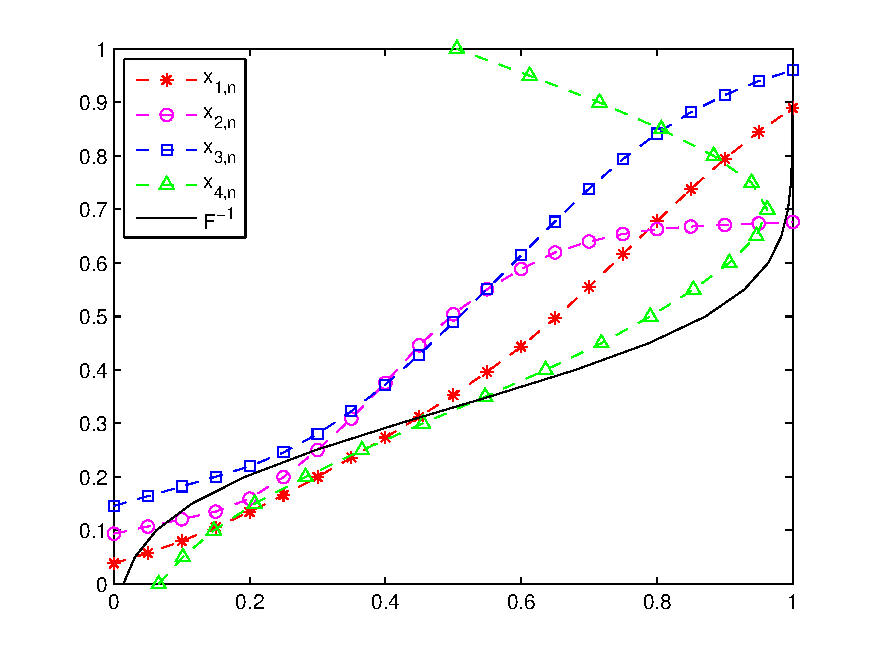
\includegraphics[width = 500pt,height = 400pt]{7.pdf}
\end{figure}






\newpage

На Рис.\ref{Pic2} представлены результаты моделирования нормально распределенной гипотетической дозы $X$ с математическим ожиданием $a_2 = 0.33$ и стандартным отклонением $b_2 = 0.3$. Выбранное среднее характеризует большую чувствительность биообъекта к препарату, что проявляется в небольших пороговых дозах, при которых наступает реакция организма. Большое значение отклонения характеризует относительно большой разброс значений величины $X$ относительно ее среднего. Объем выборки $n = 200$.

\begin{figure}[h]
\center
\caption{Результаты моделирования нормально распределенной дозы $X$ ($a=0.33$,  $b=0.3$)}\label{Pic2}
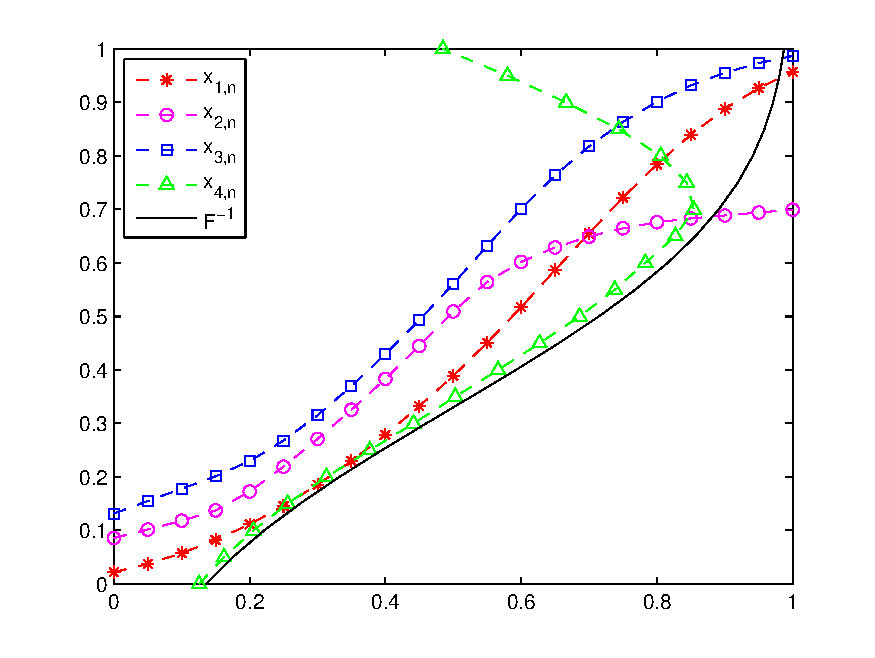
\includegraphics[width = 500pt,height = 400pt]{8.pdf}
\end{figure}

\newpage

На Рис.\ref{Pic3} представлены результаты моделирования нормально распределенной гипотетической дозы $X$ с математическим ожиданием $a_2 = 0.66$ и стандартным отклонением $b_1 = 0.15$. Выбранное среднее характеризует малую чувствительность биообъекта к препарату, что проявляется в относительно больших пороговых дозах, при которых наступает реакция организма. Малое значение отклонения характеризует небольшой разброс значений величины $X$ относительно ее среднего. Объем выборки $n = 200$.
\begin{figure}[h]
\center
\caption{Результаты моделирования нормально распределенной дозы $X$ ($a=0.66$,  $b=0.15$)}\label{Pic3}
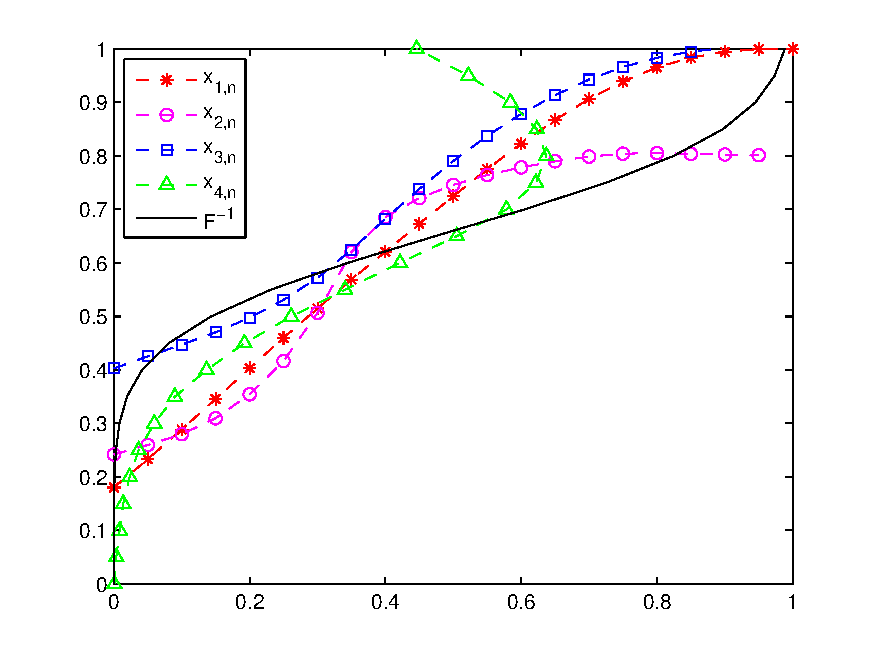
\includegraphics[width = 500pt,height = 400pt]{9.pdf}
\end{figure}

\newpage

На Рис.\ref{Pic4} представлены результаты моделирования нормально распределенной гипотетической дозы $X$ с математическим ожиданием $a_2 = 0.66$ и стандартным отклонением $b_2 = 0.3$. Выбранное среднее характеризует малую чувствительность биообъекта к препарату, что проявляется в относительно больших пороговых дозах, при которых наступает реакция организма. Большое значение отклонения характеризует относительно большой разброс значений величины $X$ относительно ее среднего. Объем выборки $n = 200$.
\begin{figure}[h]
\center
\caption{Результаты моделирования нормально распределенной дозы $X$ ($a=0.66$,  $b=0.3$)}\label{Pic4}
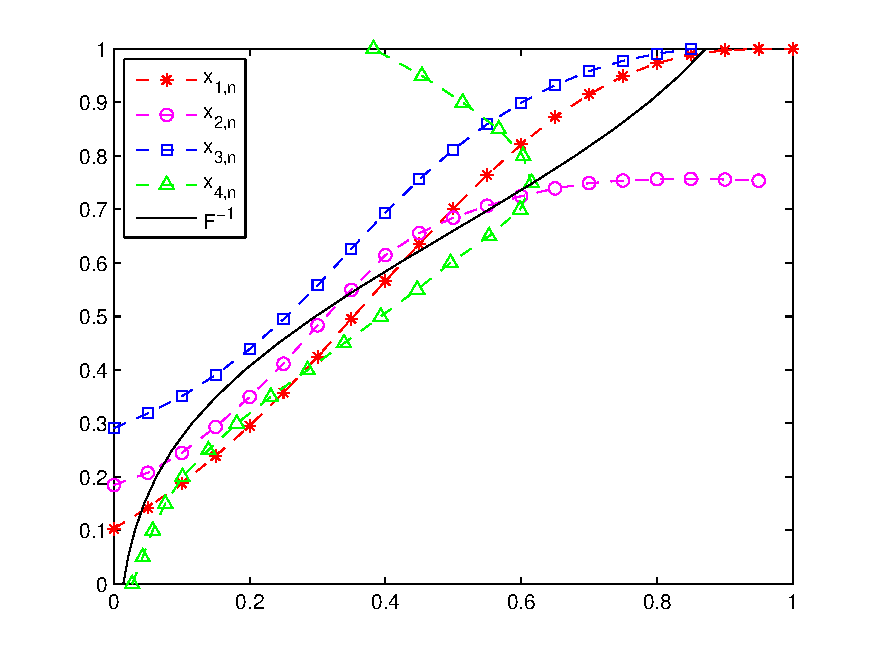
\includegraphics[width = 500pt,height = 400pt]{10.pdf}
\end{figure}
\newpage

На Рис.\ref{Pic5} представлены результаты моделирования нормально распределенной гипотетической дозы $X$ с математическим ожиданием $a_3 = 0.5$ и стандартным отклонением $b_1 = 0.15$. Выбранное среднее занимает промежуточное положение относительно средних $a_1 = 0.33$ и $a_2 = 0.66$. В данном случае пороговая доза будет принимать значения близкие к $0.5$. Разброс значений относительно математического ожидания будет небольшим за счет малости параметра $b_1$. Объем выборки $n = 200$.
\begin{figure}[h]
\center
\caption{Результаты моделирования нормально распределенной дозы $X$ ($a=0.5$,  $b=0.15$)}\label{Pic5}
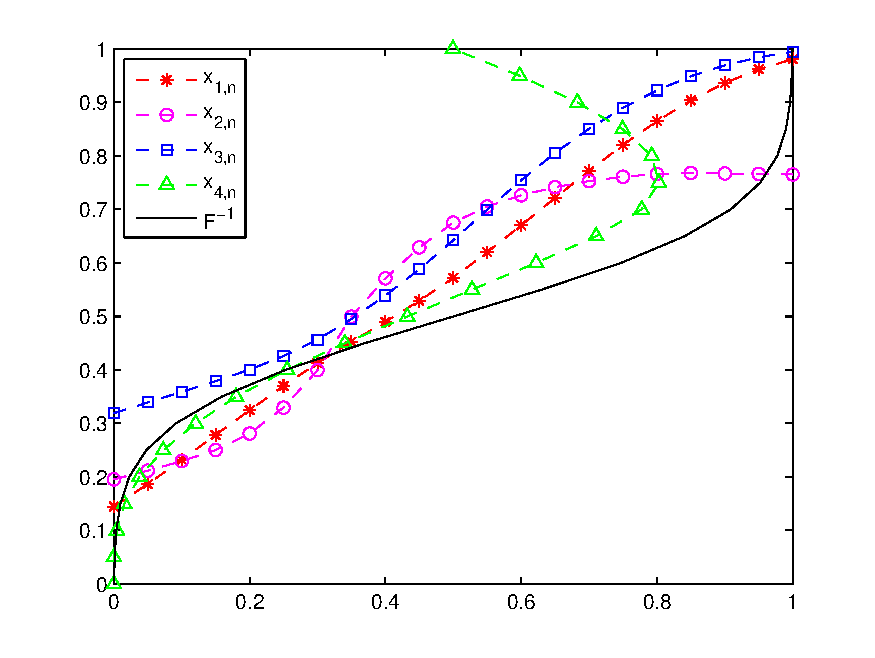
\includegraphics[width = 500pt,height = 400pt]{13.pdf}
\end{figure}
\newpage
На Рис.\ref{Pic6} представлены результаты моделирования нормально распределенной гипотетической дозы $X$ с математическим ожиданием $a_3 = 0.5$ и стандартным отклонением $b_1 = 0.3$. Выбранное среднее занимает промежуточное положение относительно средних $a_1 = 0.33$ и $a_2 = 0.66$. В данном случае пороговая доза будет принимать значения близкие к $0.5$. Разброс значений относительно математического ожидания будет значительным, поскольку стандартное отклонение $b_1$ велико. Объем выборки $n = 200$.
\begin{figure}[h]
\center
\caption{Результаты моделирования нормально распределенной дозы $X$ ($a=0.5$,  $b=0.3$)}\label{Pic6}
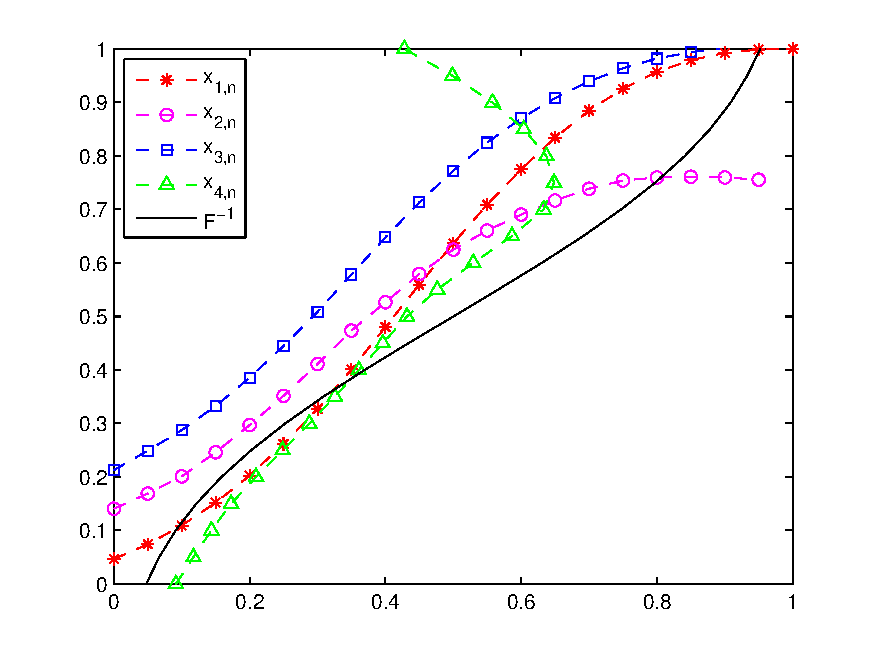
\includegraphics[width = 500pt,height = 400pt]{14.pdf}
\end{figure}
\newpage

Из рисунков \ref{Pic1} --- \ref{Pic6} видно, что в окрестности медианы распределения лучшую аппроксимацию дает естественная оценка $\hat{x}_{4,\la}$. Однако отрезок ее <<эффективного>> оценивания небольшой. Для значений пороговых доз близких к границе отрезка $[0,1]$ более удовлетворительную оценку дают величины $\hat{x}_{1,\la}$ и $\hat{x}_{3,\la}$.

На рисунках также видно положительное смещение оценок $\hat{x}_{1,\la}$, $\hat{x}_{2,\la}$, $\hat{x}_{3,\la}$ при значениях $\la$ больших математического ожидания и отрицательное (в некоторых случаях положительное, но меньшее, чем для больших $\la$) --- при меньших $\la$. Данное свойство не является следствием <<малости>> объема выборки и присуще асимптотическому поведению предложенных статистик.

Действительно, смещение оценок относительно оцениваемого квантиля $x_\la = \Fb(\la)$ определяется величинами $a_{1,r}$, $a_{2,r}$, $a_{1,d}$ и $a_{2,d}$, знаки которых положительны при $\la > E\brr{X}$. При $\la < E\brr{X}$ величины  $a_{1,d}$ и $a_{2,d}$ становятся отрицательными, однако знак суммарного смещения остается (асимптотически) положительным за счет малости $h_d$ по сравнению с $h_r$ и положительности $a_{1,r}$ и $a_{2,r}$.

Остальные результаты моделирования вынесены в приложение.

\newpage

\section*{Заключение}
% Не удаляйте следующую строчку!
\addcontentsline{toc}{section}{Заключение}
%
В работе были предложены оценки квантилей распределения пороговой дозы $X$ для модели фиксированного плана зависимости <<доза-эффект>>, доказана их состоятельность и асимптотическая нормальность.

Из предельных распределений видно, что статистики $\hat{x}_{1,\la}$ и $\hat{x}_{3,\la}$ сходятся с большей скоростью $ \sqrt{nh_r}$, чем статистика $\hat{x}_{2,\la}$ $ \sim\sqrt{nh_r^3}$.

Было проведено компьютерное моделирование эксперимента для нормального и равномерного на $[0;1]$ распределений при конечных объемах выборки: $n_1 = 50$ и $n_2=200$. Из его результатов можно сделать вывод, что для средних значений квантиля $x_\la$ лучшую аппроксимацию дает естественная оценка $\hat{x}_{4,\la}$; значения на границе отрезка $[0,1]$ лучше оценивают статистики $\hat{x}_{1,\la}$, $\hat{x}_{3,\la}$.

При анализе графиков было также выявлено (уже для конечных выборок $n_1 = 50$ и $n_2 = 200$) теоретическое асимптотическое смещение оценок относительно оцениваемого квантиля  $x_\la = \Fb(\la)$, определяемое доказанными в работе теоремами.


\newpage






\begin{thebibliography}{99}
% Не удаляйте следующую строчку!
\addcontentsline{toc}{section}{Литература}
\bibitem{Kocheganov1}  Кочеганов В.~М., Тихов М.~С. Оценивание эффективных доз в зависимости <<доза-эффект>>. --- Обозрение Прикладной и Промышленной Математики, т.18, в.1, с.85-86.
\bibitem{Kocheganov2}  Тихов М.~С., Кочеганов В.~М. Проверка гипотез согласия в зависимости <<доза-эффект>>. ---  Обозрение Прикладной и Промышленной Математики, т.18, в.1, с.187-188.
\bibitem{Krish} Криштопенко~С.В., Тихов~М.С., Попова~Е.Б. Доза-эффект.
-- M.: Медицина, 2008. -- 288 с.
\bibitem{Krish1} Криштопенко~С.В., Тихов~М.С., Попова~Е.Б. Парадоксальная токсичность. –-- Н.Новгород, изд-во НГМА, 2001 – 164 с.
\bibitem{Natan} Натансон И.~П. Теория функций вещественного переменного --- М.:~Наука, 1974.
\bibitem{Kolmogorov:1974} Колмогоров А.Н. Основные понятия теории
  вероятностей. М.: Наука, 1974. --- 119~с.
\bibitem{Kolmogorov} Колмогоров А.~Н., С.~В. Фомин Элементы теории функций и функционального анализа --- М.:~Физматилит,2006.
\bibitem{Kramer} Крамер Г. Математические методы статистики. --- М.:~Мир, 1975.
\bibitem{Gnedenko} Гнеденко Б.~В.\ Курс теории вероятностей. --- М.:~Издательство ЛКИ, 2007.
\bibitem{Shir} Липцер Р.~Ш., Ширяев А.~Н. Теория мартингалов. --- М.:~Наука, 1986.
\bibitem{Dette} Dette H., Neumeyer N., Pilz K.F. A note on nonparametric estimation of the effective dose in quantal bioassay. --- December 19, 2003.
\bibitem{Monte} Niederreiter H. Random number generation and quasi-Monte Carlo methods --- Society for industrial and applied mathematics, Philadelhia, Pennsilvania, 1992.
\bibitem{Fin} Finney, D.J. Statistical Methods in Biological Assay. Charles Griffin \& Co., 1978.




\end{thebibliography}
\newpage
\appendix
\addcontentsline{toc}{section}{Приложение}
\section*{Приложение}

\begin{figure}[h]
\center
\caption{Результаты моделирования для нормально распределенной дозы $X$, $n=50$}
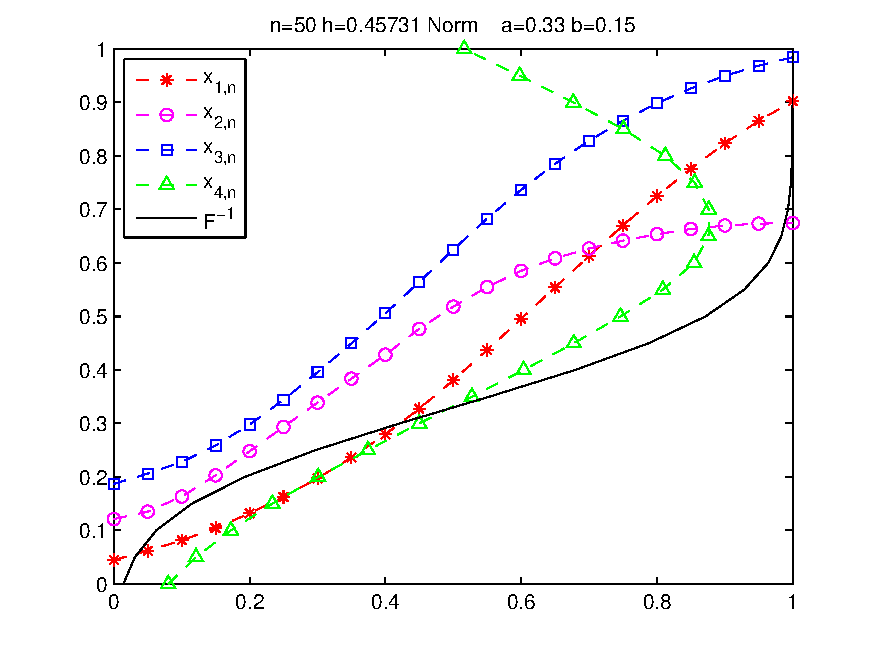
\includegraphics[width = 240pt,height = 180pt]{3.pdf}
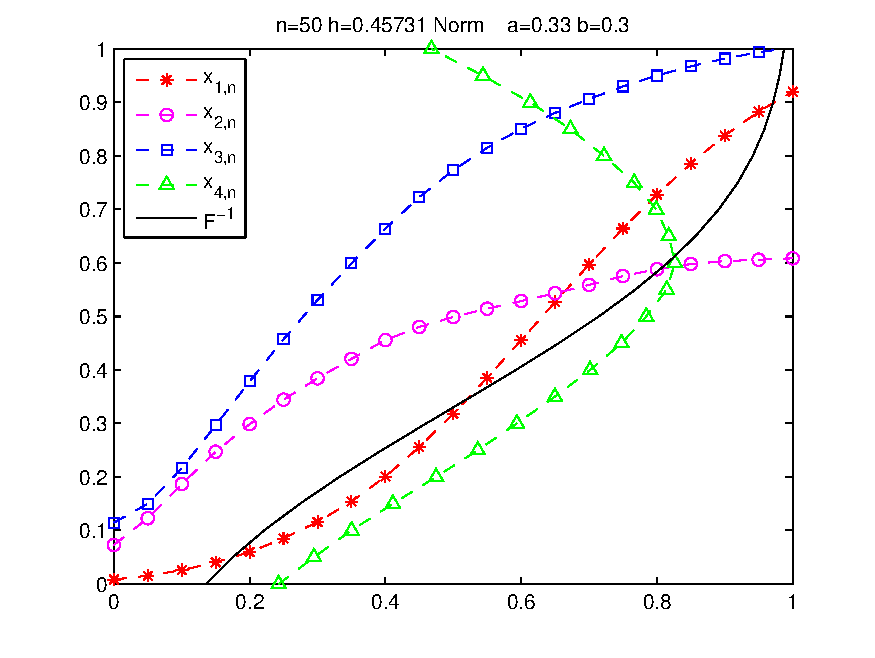
\includegraphics[width = 240pt,height = 180pt]{4.pdf}
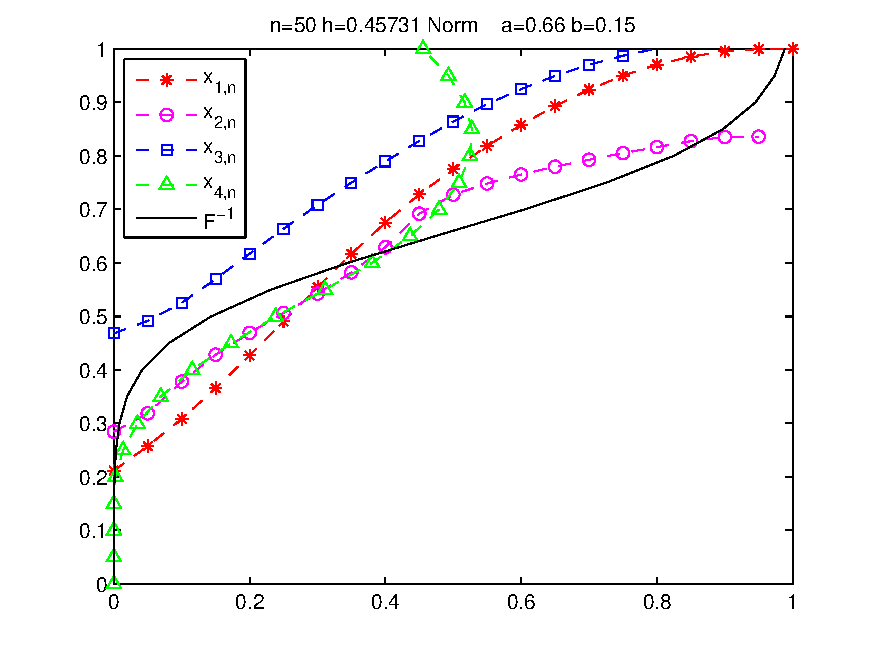
\includegraphics[width = 240pt,height = 180pt]{5.pdf}
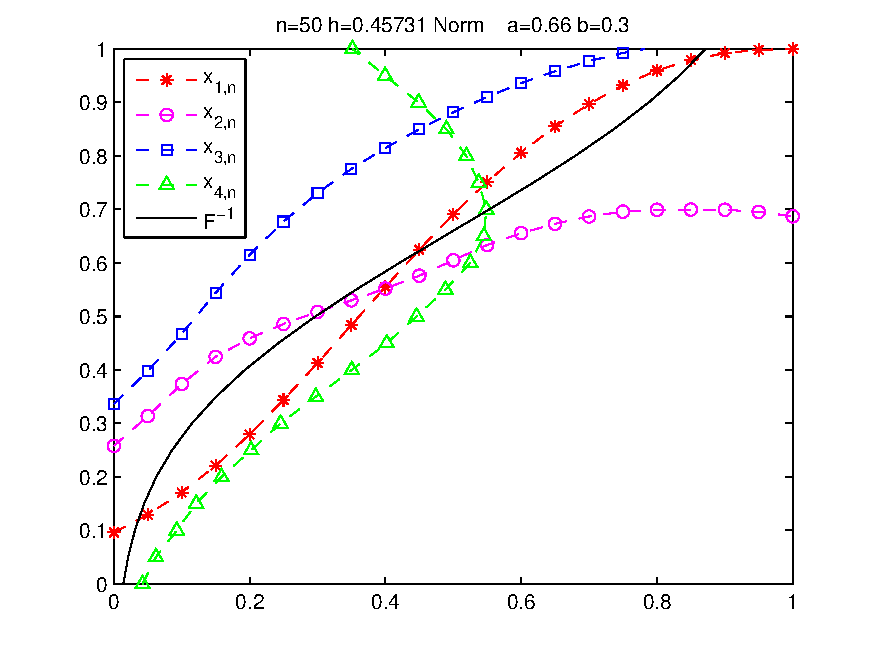
\includegraphics[width = 240pt,height = 180pt]{6.pdf}
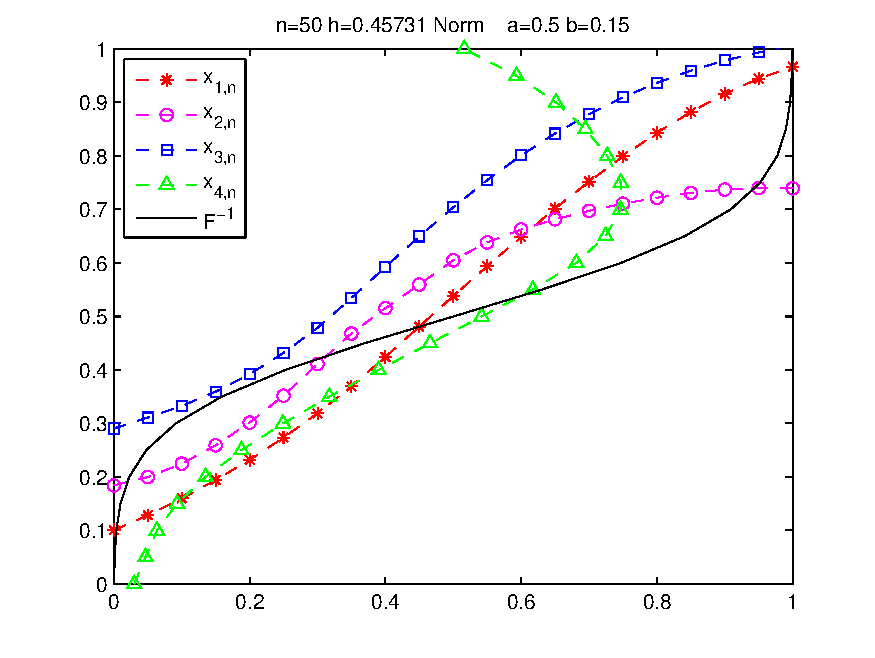
\includegraphics[width = 240pt,height = 180pt]{11.pdf}
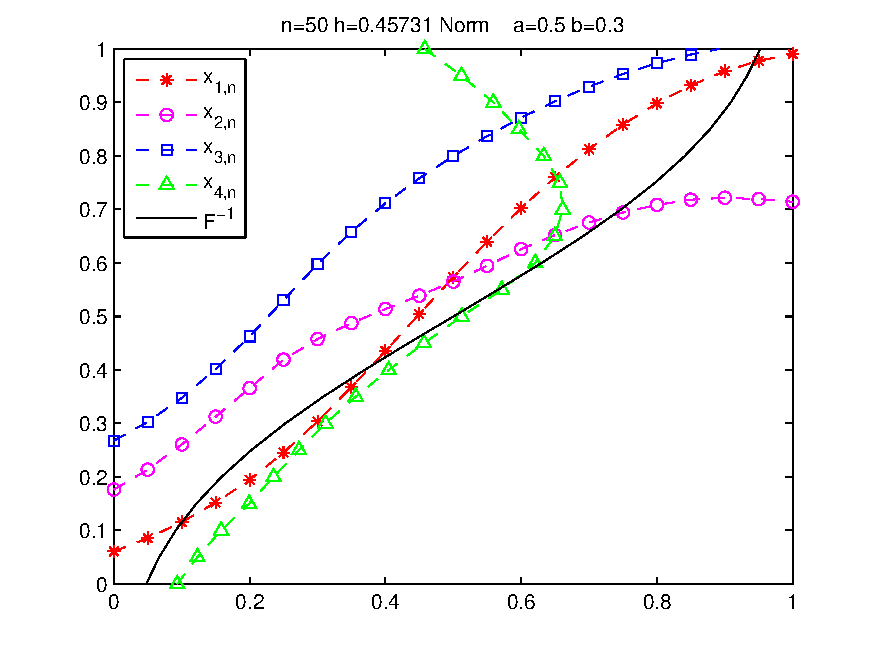
\includegraphics[width = 240pt,height = 180pt]{12.pdf}
\end{figure}

\newpage

\begin{figure}[p]
\center
\caption{Результаты моделирования для нормально распределенной дозы $X$, $n=200$}
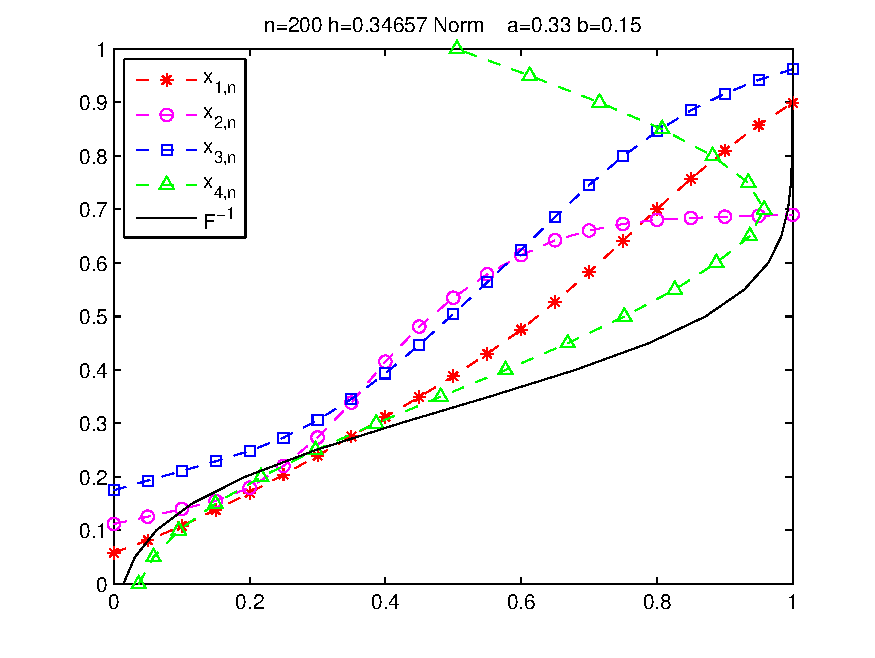
\includegraphics[width = 240pt,height = 180pt]{7n.pdf}
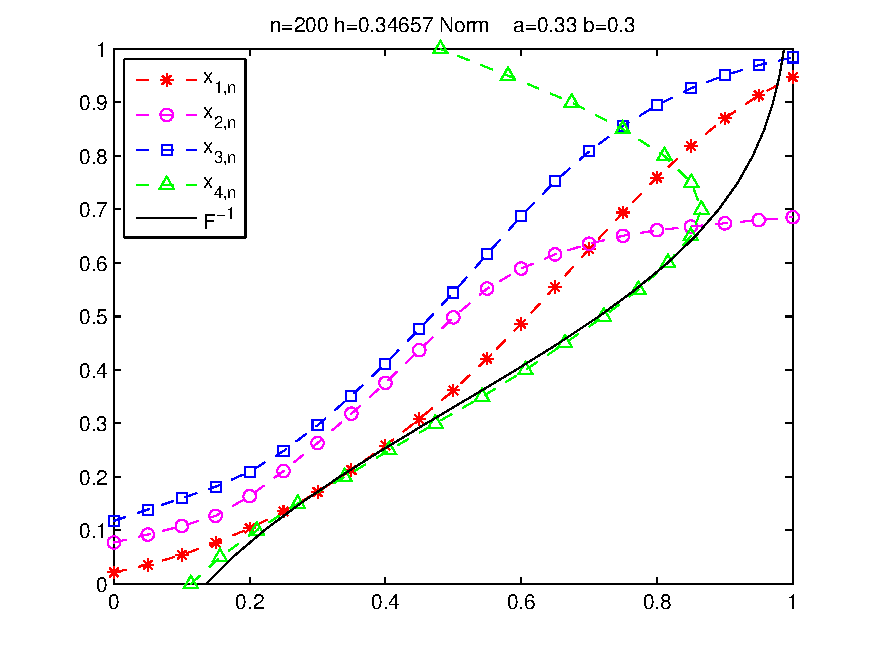
\includegraphics[width = 240pt,height = 180pt]{8n.pdf}
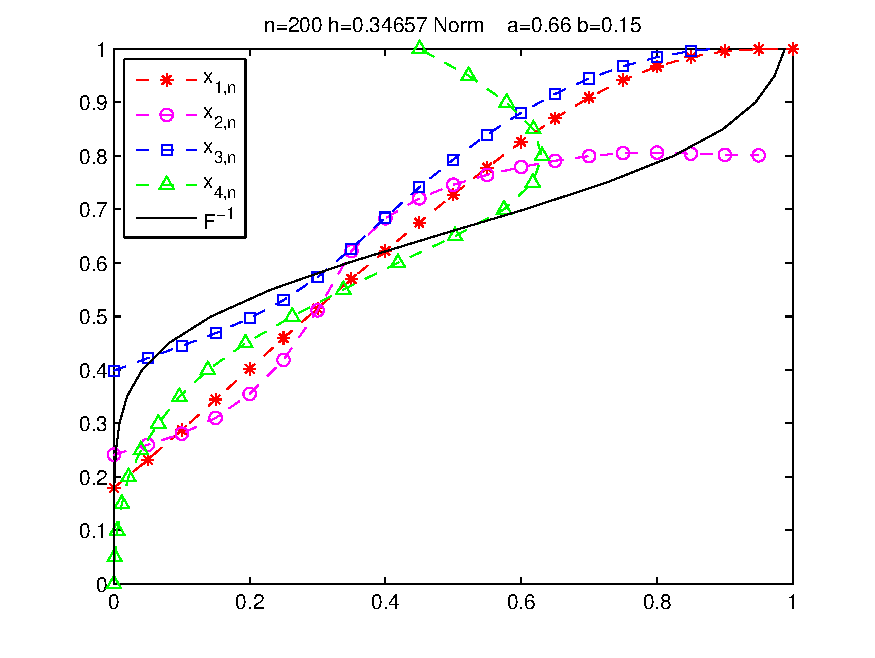
\includegraphics[width = 240pt,height = 180pt]{9n.pdf}
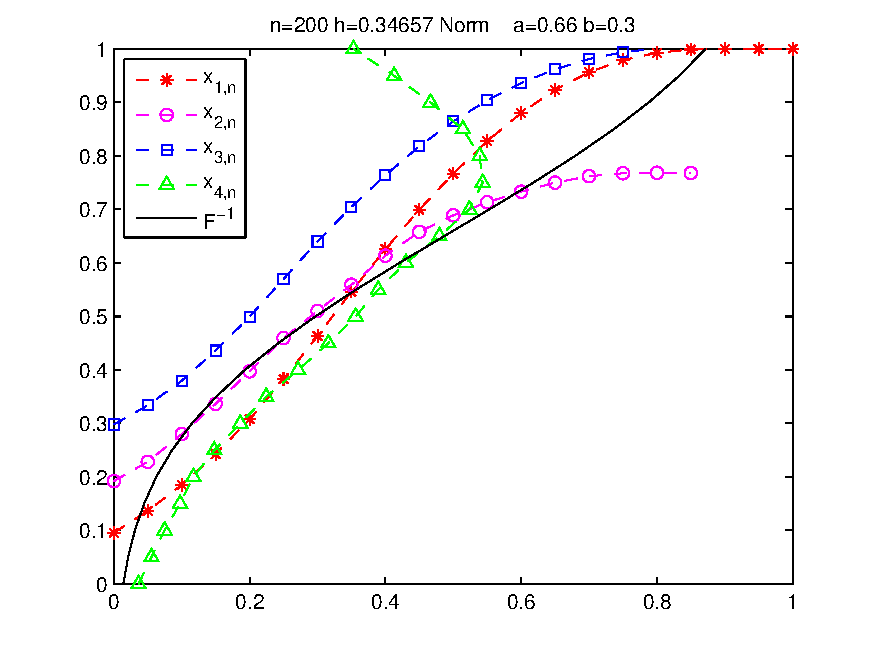
\includegraphics[width = 240pt,height = 180pt]{10n.pdf}
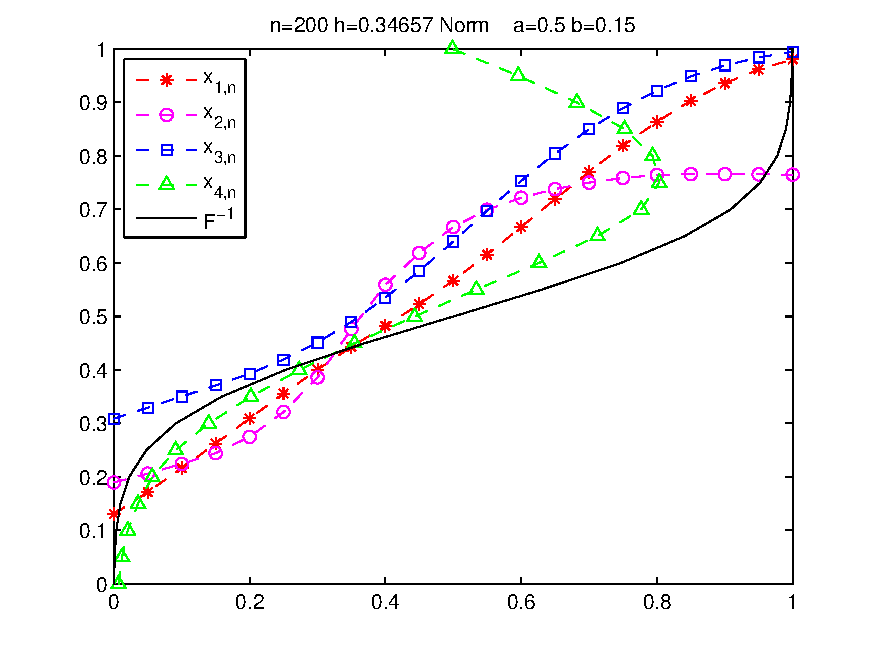
\includegraphics[width = 240pt,height = 180pt]{13n.pdf}
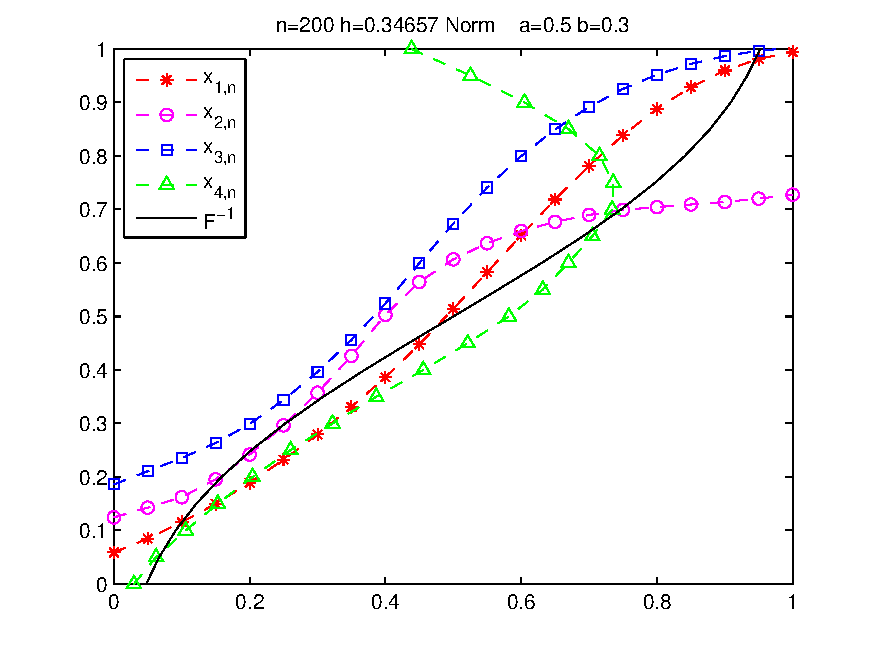
\includegraphics[width = 240pt,height = 180pt]{14n.pdf}
\end{figure}

\newpage


\begin{figure}[ht]
\center
\caption{Результаты моделирования для равномерно распределенной на $[0,1]$ дозы $X$, $n = 50$}
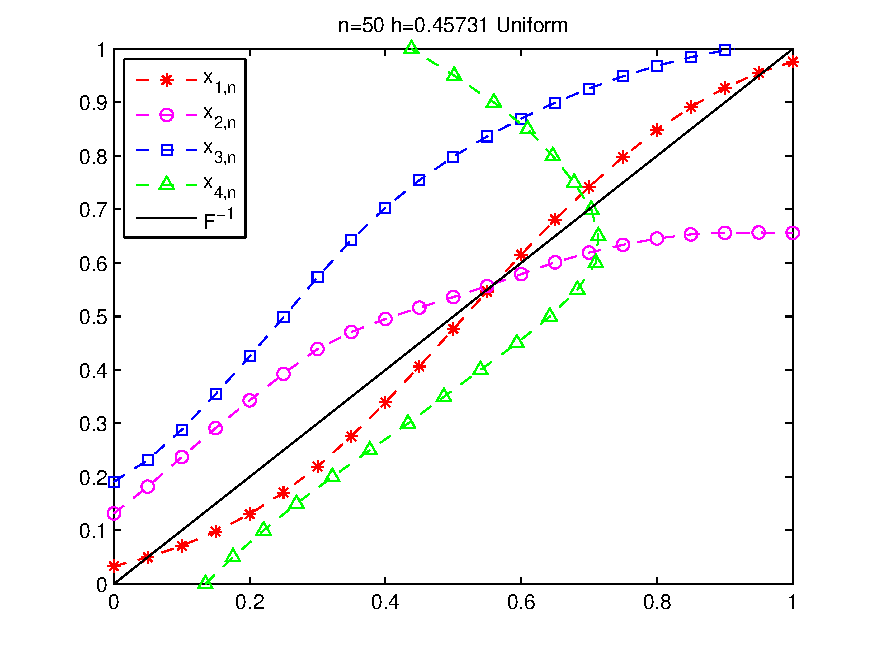
\includegraphics[width = 400pt,height = 320pt]{1.pdf}
\end{figure}

\begin{figure}[ht]
\center
\caption{Результаты моделирования для равномерно распределенной на $[0,1]$ дозы $X$, $n = 200$}
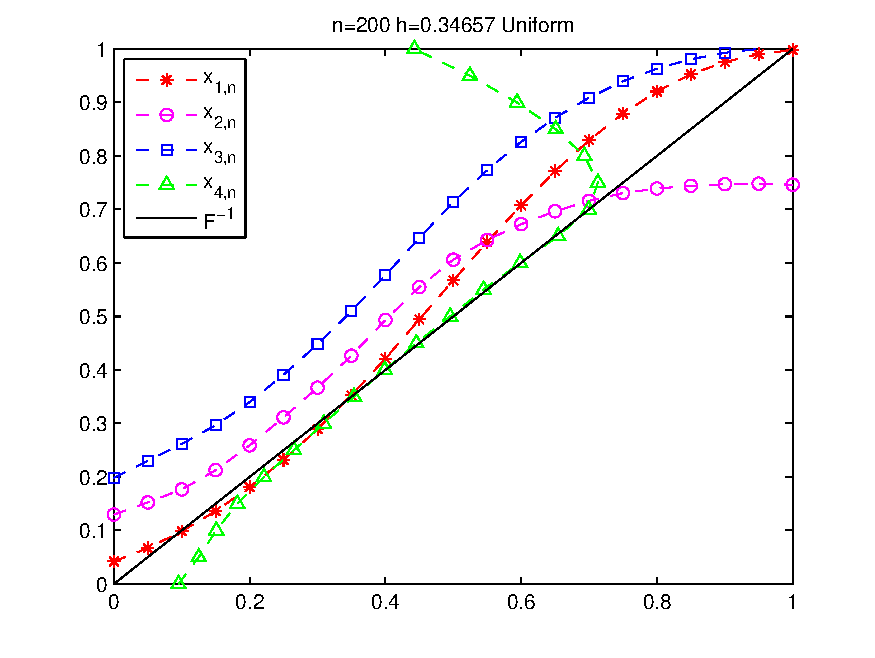
\includegraphics[width = 400pt,height = 320pt]{2.pdf}
\end{figure}



\end{document}